
\documentclass[12pt,a4paper]{article}

% ---------- 宏包 ----------
\usepackage[utf8]{inputenc}
\usepackage[T1]{fontenc}
\usepackage{amsmath,amssymb}
\usepackage{graphicx}
\usepackage{booktabs}
\usepackage{longtable}
\usepackage{array}
\usepackage{pdflscape}
\usepackage{xurl}
\usepackage{hyperref}
\usepackage[margin=1in]{geometry}
\usepackage{setspace}
\singlespacing
\usepackage[numbers,sort&compress]{natbib}
\usepackage{caption}
\usepackage{subcaption}
\usepackage{docmute}
\usepackage{enumitem}
\newcolumntype{L}[1]{>{\raggedright\arraybackslash}p{#1}}
\newcommand{\breakabletexttt}[1]{\begingroup\ttfamily\small\path{#1}\endgroup}

% ---------- 标题 ----------
\title{Validity and Robustness of LLM-Assisted Policy Simulation in Health Services Research: A Value-Sensitivity Audit}

\author{Yichao Jin \thanks{University of Texas at Dallas,Yichao.Jin@UTDallas.edu} \\
\textit{ EPPS,University of Texas at Dallas }}

\date{\today}

\begin{document}
\maketitle

% ---------- 摘要 ----------

\begin{abstract}

\noindent\textbf{Objective:} To evaluate whether LLM-assisted policy simulations are valid, robust, and normatively transparent---or whether their outputs are sensitive to model choice, prompt framing, and latent value orientations. We audit the validity of LLM-generated policy simulations in health services research using administrative burden in U.S. vaccination access as a controlled testbed.

\noindent\textbf{Study Setting and Design:} We develop a multi-level diagnostic framework for measuring normative-frame sensitivity in LLM-generated policy simulations. Fifteen LLM endpoints spanning nine provider ecosystems complete a policy-value orientation battery and simulate vaccination willingness for 27 standardized synthetic profiles (controlled test cases) under low- and high-burden conditions in a stylized U.S. vaccination-access testbed. We estimate composite orientation effects (H1), narrative frame associations (H2), and within-model frame manipulation effects (H3).

\noindent\textbf{Data Sources and Analytic Sample:} Synthetic profiles (N=27) are experimental stimuli designed to isolate how models interpret administrative-burden scenarios, not to represent a human population. H1: 15 models; H2: 2,023 profile-repetition observations; H3: 108 model--profile clusters across 2,160 observations.

\noindent\textbf{Principal Findings:} 
(1) Composite orientation--effect: PVOC coefficient $\beta_1 = 1.51$, 95\% CI [$-$2.41, 5.43], $p = 0.45$---composite orientation does not predict cross-model variation.
(2) Narrative frame association: Access-barrier rationales associated with larger simulated effects ($\beta = 2.34$, 95\% CI [0.87, 3.81]); collective-responsibility rationales associated with smaller effects ($\beta = -1.89$, 95\% CI [$-$3.12, $-$0.66]).
(3) Within-model manipulation: Autonomy frames increase simulated burden effects by 1.8 percentage points (95\% CI [0.4, 3.2]); collective-obligation frames reduce effects by 2.1 percentage points (95\% CI [$-$3.5, $-$0.7]).

\noindent\textbf{Conclusions:} LLM-assisted policy simulation is normatively frame-sensitive. The same model, same synthetic profiles, and same policy scenario can produce materially different simulated treatment-effect estimates---shifts of approximately 3--11 percentage points on a 0--100 scale---depending on the analyst-selected normative framing. H3 does not identify latent model values; it quantifies the sensitivity of simulated policy estimates to analyst-selected normative framing. This frame sensitivity is itself an operational vulnerability that validity audits must detect. Researchers should audit simulation validity before deploying LLMs as policy-simulation tools in HSR.

\vspace{0.5em}
\noindent\rule{\textwidth}{0.4pt}
\vspace{0.3em}

\noindent\textbf{What is known on this topic}
\begin{itemize}[leftmargin=*,noitemsep,topsep=0pt]
\item LLMs are increasingly used to simulate social judgments and policy effects in health services research.
\item Prior work measures model values through direct survey prompts rather than downstream simulated policy effects.
\item Less is known about whether latent value orientations shape simulated treatment effects under policy conditions.
\end{itemize}

\vspace{0.3em}
\noindent\textbf{What this study found}
\begin{itemize}[leftmargin=*,noitemsep,topsep=0pt]
\item Composite policy-value scores do not predict cross-model variation in simulated burden effects.
\item Narrative interpretive frames (access-barrier, collective-responsibility) are systematically associated with simulated effect sizes.
\item Within-model frame manipulation confirms: autonomy and equity/access frames increase simulated burden effects; collective-obligation frames reduce them.
\item LLM-assisted policy simulation requires systematic validity auditing before deployment in HSR.
\end{itemize}

\end{abstract}

% ---------- 关键词 ----------
\noindent\textbf{Keywords:} large language models, simulation validity, administrative burden, policy simulation robustness, normative-frame sensitivity, calibration

% ---------- 正文 ----------
% ---------- Introduction 部分引用的文献 ----------

\section{Introduction}

Administrative burden in U.S. health services---the learning, psychological, and compliance costs that individuals face when interacting with public programs---is a well-documented barrier to care \citep{Shin2025}. These burdens include forms, documentation requirements, waiting time, procedural uncertainty, and perceived loss of autonomy, and they can delay or discourage access to vaccination and other preventive services \citep{Shin2025}. Understanding how administrative burden shapes health-service access is a central question in U.S. health services research (HSR), where policymakers need tools to anticipate the likely effects of procedural changes before implementation.

Large language models (LLMs) are increasingly used in HSR not only to generate text but also to simulate social judgments, preferences, and behavioral responses \citep{Aher2022,Park2023,Argyle2023,Lin2024}. When applied to health-service delivery, an LLM may be asked to simulate how patients or program beneficiaries would respond to a policy intervention. This creates a methodological chain:
\[
\text{administrative burden} \rightarrow \text{health-service access/delivery} \rightarrow \text{LLM policy simulation} \rightarrow \text{validity threat from analyst framing}.
\]
The core validity question is whether LLM-assisted policy simulations are robust across models and framing choices---or whether their outputs are sensitive to the normative lens activated by model architecture, training data, or prompt design. This is a simulation validity question for U.S. health services research: if the same administrative-burden scenario produces substantially different predicted effects depending on which model is used and how the prompt is framed, then LLM-assisted policy simulation requires systematic auditing before it can be trusted as an HSR methodology.

Vaccination access in the U.S. provides a controlled HSR testbed for evaluating this validity threat. Administrative burden intersects with individual choice, public health externalities, institutional trust, and procedural barriers---properties that make it well-suited for detecting whether simulation outputs are valid and robust across models and frames. The U.S. context is particularly relevant given ongoing policy debates about vaccine mandates, administrative requirements for immunization programs, and health equity in access to preventive care.

This paper evaluates whether LLM-assisted policy simulations are valid, robust, and normatively transparent---or whether their outputs are sensitive to model choice, prompt framing, and latent value orientations. The core question is not whether models state particular political opinions, but whether their simulated treatment effects are sensitive to the normative lens activated by the model's architecture, training data, or prompt design.

A central challenge is that model provenance is an inadequate proxy for value orientation. To avoid treating development origin as a fixed ideological category, I independently measure each model's policy-value orientation using a structured battery capturing five dimensions: autonomy protection, state trust, collective obligation, administrative-burden sensitivity, and coercion aversion.

The study addresses three research questions. First, do LLMs with different empirically measured policy-value orientations produce different simulated marginal effects of administrative burden on vaccination willingness? Second, are simulated burden effects systematically associated with the interpretive frames used in model rationales? Third, can simulated burden effects be shifted within the same base model by experimentally assigning governance-value frames?

Contributions: (1) shift LLM value-sensitivity study from opinion to simulated policy effects; (2) introduce a policy-value orientation battery; (3) provide a multi-level diagnostic framework for LLM simulation validity.

\section{Theoretical Framework and Hypotheses}


\subsection{Policy-Value Orientation}
\label{sec:orientation-effect}

I define a model's \textit{policy-value orientation} as its systematic tendency to interpret governance situations through assumptions about individual--institution relationships, legitimacy of public authority, and acceptability of procedural costs. In administrative-burden settings, these assumptions matter because the same procedural requirement can be interpreted as a legitimate safeguard, an access barrier, an infringement on autonomy, or a reasonable cost of collective protection.

The framework focuses on five dimensions: autonomy protection, state trust, collective obligation, administrative-burden sensitivity, and coercion aversion. These dimensions are operationalized through a structured orientation battery (Section~\ref{sec:orientation-battery}). The composite PVOC (Policy-Value Orientation Composite) aggregates the five dimensions with theoretically specified directional weights, but is treated as a theory-specified diagnostic aggregate rather than a validated psychometric scale, consistent with prior evidence that aggregate composites can produce unstable estimates in small model samples.

\emph{Measurement diagnostics.} Internal consistency is mixed: only collective obligation reaches conventional reliability ($\alpha = 0.869$). This limitation is consistent with prior findings that psychometric scales designed for humans may not transfer directly to LLMs \citep{Rottger2024}, underscoring why the composite analysis must be interpreted alongside dimension-specific and frame-level evidence.

\subsection{Hypotheses}
\label{sec:hypotheses}

The empirical tests proceed in three linked steps, moving from an aggregate orientation index to narrative-level associations to within-model causal evidence. The tests form a diagnostic framework rather than a single confirmatory chain: each step is informative regardless of the outcome of the preceding one.

\textbf{H1 (Composite Orientation--Effect).} If LLM policy simulations are systematically influenced by latent policy-value orientations, then models with higher composite PVOC scores (Policy-Value Orientation Composite, indexing autonomy protection, burden sensitivity, and coercion aversion against state trust and collective obligation) should produce larger simulated administrative-burden effects on vaccination willingness. A null result would imply that value sensitivity, if present, does not follow a simple composite pathway, suggesting the need for more granular diagnostics such as narrative frame decomposition or experimental manipulation.

\textbf{H2 (Narrative Frame Association).} Interpretive frames expressed in model rationales are expected to be systematically associated with simulated burden effects, independent of the composite PVOC. Access-barrier, autonomy-infringement, and coercive-backlash frames are expected to correspond to larger simulated burden effects; procedural-legitimacy and collective-responsibility frames are expected to correspond to smaller effects. Because frames are generated by the model rather than experimentally assigned, H2 identifies descriptive associations rather than causal pathways.

\textbf{H3 (Frame Manipulation).} Randomly assigning governance-value frames to the same base model is expected to causally shift simulated burden effects relative to a neutral frame. Autonomy and equity/access frames are expected to increase simulated burden effects, while collective-obligation frames are expected to decrease them. Because the base model, profiles, scenarios, and output format are held fixed, any shift in simulated effects can be attributed to the frame itself rather than to stable model characteristics.

\medskip
\noindent The three hypotheses are designed as a diagnostic framework rather than a sequential gamble. Each addresses a distinct question---aggregate orientation, narrative association, and causal frame---and each is informative whether or not the others yield significant results.

\begin{figure}[htbp]
\centering
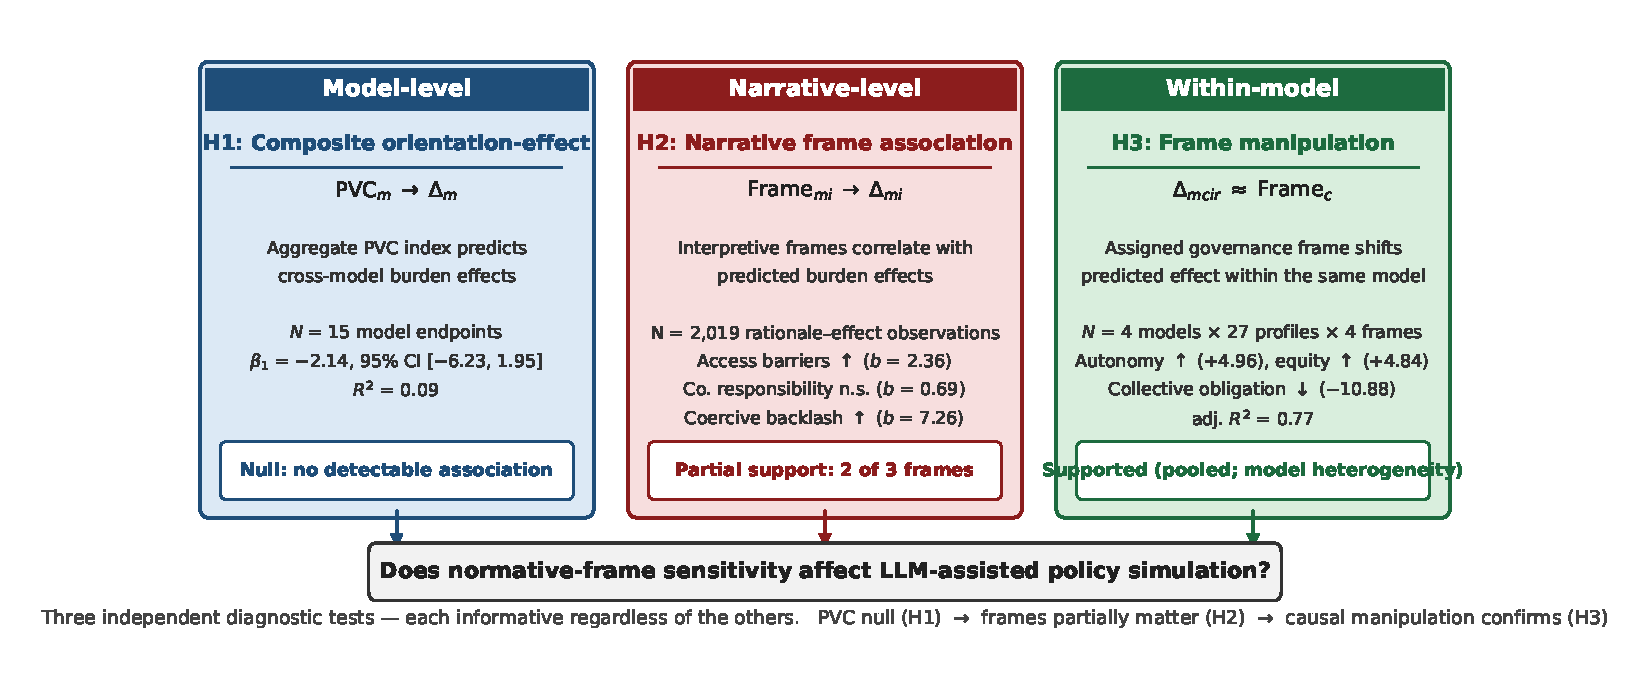
\includegraphics[width=\textwidth]{fig1_conceptual.pdf}
\caption{Diagnostic framework for three levels of value sensitivity testing. H1 tests whether a model-level PVOC predicts cross-model variation in administrative-burden effects. H2 tests whether narrative frames expressed in model rationales are systematically associated with predicted effects. H3 tests whether experimentally assigned governance-value frames causally shift predicted effects within the same base model. The three tests are designed as independent diagnostic components: each is informative regardless of the outcome of the others.}
\label{fig:conceptual}
\end{figure}

\section{Experimental Design and Methods}

\subsection{Model Sample}
\label{subsec:model-sample}

We evaluate fifteen LLM endpoints spanning nine provider ecosystems: OpenAI, Anthropic, Google, Meta, Mistral, Cohere, Moonshot AI, DeepSeek, and Qwen. The original nine-model sample included GPT-4.1, GPT-4.1 mini, GPT-4o, Claude Sonnet 4.6, Gemini 2.5 Pro, Gemini 2.5 Flash, Llama 3.1 70B Instruct, DeepSeek-V3.2, and Qwen3.6-72B-Instruct. To expand cross-model coverage, we added six endpoints accessed through OpenRouter: Claude Opus 4.8, Claude Haiku, Llama 3.1 8B Instruct, Mistral Large, Cohere Command R+, and Kimi K2.6. The sample is intentionally heterogeneous to cover frontier proprietary, lower-cost, hosted open-weight, enterprise-oriented, and non-U.S. ecosystems; it supports cross-model auditing but not provider-level causal comparisons. All models were run with temperature set to zero where supported, and each model--scenario--profile cell was repeated five times in fresh contexts. Detailed model identifiers and decoding parameters are reported in the Online Supplement.

\subsection{Policy-Value Orientation Battery}
\label{subsec:orientation-battery}

We administered a 20-item Likert battery measuring five dimensions: autonomy protection, state trust, collective obligation, administrative-burden sensitivity, and coercion aversion. Each dimension uses four items on a 1--7 scale. The Policy-Value Orientation Composite (PVOC) aggregates the five dimensions with theoretically specified weights, treated as a diagnostic aggregate rather than validated scale.

\subsection{Administrative-Burden Simulation}
\label{subsec:burden}

To measure each model's simulated burden effect, we designed a vaccination-access simulation as a controlled HSR testbed, in which the same standardized profile faces two policy conditions: low administrative burden and high administrative burden. The simulation was administered after the orientation battery but before any frame manipulation, using a fresh API call for each model--profile--condition--repetition.

\subsubsection{Standardized synthetic profiles (controlled test cases)}
\label{subsub:profiles}

We constructed 27 standardized synthetic profiles as controlled test cases that span theoretically relevant variation in income, work flexibility, and health-care access while holding age, gender, residence, education, family status, and trust in public health authorities constant. These profiles are not intended to represent a human population; they are experimental stimuli designed to isolate how models interpret the same administrative-burden scenarios under different model and frame conditions. The full profile set is reported in the Online Supplement.

\subsubsection{Low- and high-burden scenarios}
\label{subsub:scenarios}

For each standardized profile, we defined two burden levels that differ in the administrative requirements for obtaining a vaccination. The low-burden condition involves online appointment scheduling, a nearby pharmacy with extended hours, no documentation beyond identification, and an estimated total time of 15 minutes. The high-burden condition simultaneously increases multiple procedural costs: in-person registration at a designated public health center, required income verification and proof of residency, paper forms, an estimated waiting time of 1--2 hours, and an appointment required at least one week in advance.

These scenarios are designed as a \textbf{stylized U.S. vaccination-access testbed} for auditing LLM simulation validity, not as a realistic representation of any specific U.S. vaccination program. The high-burden condition intentionally bundles multiple administrative barriers to create a controlled contrast for testing model sensitivity; it does not estimate the magnitude of administrative burden in any actual health service delivery setting. The income verification and residency requirements are included as stylized procedural barriers typical of means-tested public programs, not because they reflect realistic vaccination access requirements. Full prompt templates are provided in the Online Supplement.

\subsubsection{Outcome: predicted willingness and marginal burden effect}
\label{subsub:burden-outcome}

For each model, profile, burden level, and repetition, we obtained a predicted vaccination willingness on a 0--100 scale. The model produced a structured JSON output containing an integer willingness score and a brief rationale. The primary outcome is the marginal effect of moving from low to high burden for a given model, profile, and repetition: \(\Delta_{mir} = W_{mi,\text{low},r} - W_{mi,\text{high},r}\). Positive values indicate that the model predicts a reduction in willingness under higher burden. For model-level analyses, we average across profiles and repetitions.

\subsection{Task-Compliance Diagnostics}
\label{subsec:capability}

Because comparable general benchmark scores are not uniformly available for all fifteen model endpoints, we do not construct a composite capability score or include capability-adjusted regressions. Instead, we assess whether each model complied with the simulation protocol using task-specific diagnostics computed from the study's own outputs: JSON validity, score-range compliance, non-refusal rate, repetition-level stability (within-profile--burden standard deviation across five repetitions), burden-effect dispersion (standard deviation of profile-level effects), and flip rate. These diagnostics, reported in Table~\ref{tab:data_quality}, verify protocol compliance and output stability rather than construct a general capability ranking. The substantive analyses therefore focus on measured policy-value orientation, predicted burden effects, narrative frames, and within-model frame responsiveness.

\subsection{Narrative coding framework}
\label{subsec:narrative-coding}

To test whether interpretive frames account for the relationship between policy-value orientation and predicted burden effects (H2), we coded the rationales generated during the administrative-burden simulation. The coding framework contains five theoretically derived frames: \emph{autonomy infringement} (procedures framed as threats to individual choice or procedural dignity), \emph{procedural legitimacy} (administrative requirements framed as justified safeguards), \emph{collective responsibility} (civic duty and tolerance of inconvenience for public health), \emph{access barriers} (procedural costs framed as disproportionately burdening disadvantaged groups), and \emph{coercive backlash} (mandates or penalties expected to generate resistance).

Each rationale consists of one to three sentences generated in the structured output. Rationales are de-identified before coding. We apply a rule-based algorithm to code each rationale into five interpretive frames using predefined keyword patterns (regular expressions) derived from the theoretical framework. The algorithm matches case-insensitive text patterns corresponding to each frame definition; a frame is coded as present (1) if any pattern matches, absent (0) otherwise. Frames are non-mutually exclusive---a single rationale may contain multiple frames. The full pattern dictionary and validation protocol are reported in the Online Supplement.

For validation, a random sample of 200 rationales (approximately 10\% of the high-burden sample) was manually inspected to confirm that pattern assignments reflected the codebook definitions rather than superficial keyword matches. This validation focused especially on access-barrier coding, where generic mentions of paperwork or waiting time are not sufficient for a positive code. The manual inspection confirmed pattern validity; no systematic misclassification patterns were identified that would require pattern refinement.

For each model, profile, and repetition, each frame is recorded as a binary indicator equal to one if the rationale contains at least one instance of that frame. These binary frame indicators are used in the frame-decomposition analysis as descriptive evidence of rationale--outcome co-expression rather than definitive causal mediation, because model-level policy-value orientation is measured rather than experimentally assigned.

\subsection{Within-Model Frame Manipulation}
\label{sec:frame-manipulation}

To test whether governance-value frames systematically shift predicted burden effects (H3), we conducted a within-model experiment in which the same base model was exposed to different system-prompt frames before completing the burden simulation. The assigned frame is experimentally varied while the base model, synthetic profiles, burden scenarios, output format, and decoding settings are held fixed. This design provides within-model evidence that framing can influence simulated burden effects. Because API-hosted models may still be affected by hidden alignment, provider-side routing, or residual stochasticity, we do not interpret the manipulation as identifying a permanent change in model values.

\subsubsection{Model selection}

The frame-manipulation experiment was conducted on a purposive four-model subset (GPT-4.1, Llama 3.1 70B Instruct, Qwen3.6-72B Instruct, and Mistral Large) representing a frontier proprietary closed-source model, a hosted open-weight model, a non-U.S. model ecosystem, and a low-PVOC robustness case. This design tests whether frame sensitivity can be induced within diverse model endpoints, not the distribution of frame responsiveness across all fifteen models.

\subsubsection{Frame conditions and randomization}

Four system-prompt frames were used: \emph{neutral}, \emph{autonomy} (weighting individual choice, privacy, and procedural dignity), \emph{collective obligation} (weighting civic responsibility and public health coordination), and \emph{equity/access} (weighting unequal procedural costs and barriers faced by disadvantaged groups). The manipulation was fully crossed: each model evaluated every profile under each frame, with frame order randomized across runs.

\subsubsection{Statistical analysis}

To test whether the assigned frame shifts \(\Delta\), we estimate the burden effect with model and profile fixed effects, and indicator variables for each value frame (neutral as the reference category), adjusting pairwise comparisons using the Holm--Bonferroni correction. Because the frame manipulation is fully crossed within each model, profile fixed effects are identified within-model and absorb all time-invariant profile-level heterogeneity. Standard errors are clustered at the profile level to account for the five repeated queries per profile, treating the profile as the primary sampling unit. The inferential target is the profile-level frame contrast, not a population-level treatment effect. Full results are reported in Section~\ref{subsubsec:results-h3} and the Online Supplement.
\subsection{Estimation Strategy}
\label{sec:estimation}

We test H1--H3 using hypothesis-specific estimation strategies. Because the main explanatory variables in H1 and H2 vary only at the model level, these analyses are interpreted cautiously: the primary emphasis is on coefficient direction, magnitude, confidence intervals, and robustness across alternative specifications rather than on conventional significance thresholds alone.

\subsubsection{Orientation-effect models (H1)}
\label{sec:est-h1}

The primary H1 analysis tests whether models with higher PVOC scores predict larger burden effects:
\[
\bar{\Delta}_m = \beta_0 + \beta_1 \text{PVOC}_m + \epsilon_m,
\]
where \(\bar{\Delta}_m\) is the average burden effect across profiles and repetitions. Because the identifying variation in PVOC exists only at the model level, this analysis is interpreted as a descriptive cross-model association rather than a high-powered population estimate. We also estimate separate bivariate regressions replacing the composite PVOC with each of the five orientation dimensions (autonomy protection, state trust, collective obligation, administrative-burden sensitivity, and coercion aversion) as diagnostic checks, not as confirmatory tests of validated subscales.

\subsubsection{Narrative frame-decomposition models (H2)}
\label{sec:est-h2}

The H2 analysis decomposes associations between PVOC, expressed rationale frames, and predicted burden effects at the model--profile level. We refer to this as ``mediation-style'' because PVOC is measured rather than randomized and varies only at the model level; the estimates should be interpreted as frame--outcome association diagnostics rather than formal causal mediation. The H2 product terms summarize whether models with different PVOC scores tend to express different frames and whether those expressed frames are associated with different predicted burden effects. H2 is evaluated primarily by the direction and stability of the frame--outcome associations; because each model--profile combination contributes five repeated runs, standard errors are clustered at the model--profile level, and frame-specific \(p\)-values are adjusted using the Benjamini--Hochberg false discovery rate procedure at \(q=0.10\).

\subsubsection{Frame-manipulation models (H3)}
\label{sec:est-h3}

Using the within-model frame-manipulation data, we estimate a two-way fixed-effects model:
\[
\Delta_{mcir} = \alpha_m + \mu_i + \beta_1 \mathbb{I}(c=\text{Autonomy}) + \beta_2 \mathbb{I}(c=\text{Collective}) + \beta_3 \mathbb{I}(c=\text{Equity}) + \varepsilon_{mcir},
\]
with neutral as the omitted reference, model fixed effects \(\alpha_m\), and profile fixed effects \(\mu_i\). Pairwise comparisons against the neutral frame are adjusted using the Holm--Bonferroni correction, and model-specific frame effects are reported separately. Because each model--profile--frame cell contains five repeated runs, standard errors are clustered at the model--profile level to account for within-cell correlation across repetitions.

\subsubsection{Multiple-testing and robustness checks}
\label{sec:robustness}

Within hypothesis families, we apply the Benjamini--Hochberg FDR procedure at \(q=0.10\) for H2 (five frames) and the Holm--Bonferroni correction for H3 (three value frames). H1's primary test concerns a single coefficient, so no adjustment is applied. Robustness checks exclude each synthetic profile one at a time; replace PVOC with its five separate dimension scores; use an unweighted raw-score PVOC; use binary frame presence rather than intensity in H2; and exclude models below alternative willingness thresholds.

\section{Results}

\subsection{Data Quality and Descriptive Statistics}
\label{sec:results-data-quality}

Table~\ref{tab:data_quality} reports task-compliance diagnostics for the expanded fifteen-model simulation (4,050 raw responses, 2,025 low--high burden-effect pairs). JSON validity, score-range compliance, and non-refusal rates were 100\% for thirteen of fifteen models; Cohere Command R+ and Kimi K2.6 each had one malformed response (99.6\% compliance). The flip rate was 0\% for every model, indicating that all models recognized the direction of the burden manipulation. Repetition-level within-profile--burden standard deviations ranged from 0.00 to 3.18 points on the 0--100 scale, indicating high within-model stability. Mean predicted willingness varied substantially across models (51.61--71.61), motivating the use of the within-profile marginal burden-effect outcome in the main analyses.

\begin{table}[htbp]
\centering
\caption{Data quality and simulation diagnostics by model}
\label{tab:data_quality}
\setlength{\tabcolsep}{4pt}
\resizebox{\textwidth}{!}{%
\begin{tabular}{lrrrrrrrr}
\toprule
Model & \(N\) & JSON\% & Score\% & NonRef\% & Mean \(W\) & StabSD & DeltaSD & Flip\% \\
\midrule
GPT-4o & 270 & 100.0 & 100.0 & 100.0 & 71.61 & 0.43 & 7.13 & 0.0 \\
GPT-4.1 & 270 & 100.0 & 100.0 & 100.0 & 68.30 & 0.62 & 7.12 & 0.0 \\
Llama 3.1 8B & 270 & 100.0 & 100.0 & 100.0 & 65.41 & 0.28 & 4.54 & 0.0 \\
Llama 3.1 70B & 270 & 100.0 & 100.0 & 100.0 & 64.70 & 0.37 & 9.75 & 0.0 \\
Qwen3.6-72B & 270 & 100.0 & 100.0 & 100.0 & 61.57 & 3.18 & 7.22 & 0.0 \\
Mistral Large & 270 & 100.0 & 100.0 & 100.0 & 60.73 & 0.88 & 5.41 & 0.0 \\
Cohere Command R+ & 270 & 99.6 & 99.6 & 100.0 & 60.32 & 1.52 & 4.77 & 0.0 \\
GPT-4.1 mini & 270 & 100.0 & 100.0 & 100.0 & 58.96 & 0.87 & 3.86 & 0.0 \\
Gemini 2.5 Flash & 270 & 100.0 & 100.0 & 100.0 & 58.91 & 1.57 & 9.05 & 0.0 \\
Kimi K2.6 & 270 & 99.6 & 99.6 & 100.0 & 58.25 & 1.39 & 5.83 & 0.0 \\
Claude Haiku & 270 & 100.0 & 100.0 & 100.0 & 56.85 & 0.00 & 6.59 & 0.0 \\
Gemini 2.5 Pro & 270 & 100.0 & 100.0 & 100.0 & 55.50 & 2.49 & 5.83 & 0.0 \\
Claude Opus 4.8 & 270 & 100.0 & 100.0 & 100.0 & 53.03 & 0.77 & 6.15 & 0.0 \\
DeepSeek-V3.2 & 270 & 100.0 & 100.0 & 100.0 & 52.07 & 0.96 & 4.48 & 0.0 \\
Claude Sonnet 4.6 & 270 & 100.0 & 100.0 & 100.0 & 51.61 & 0.46 & 5.72 & 0.0 \\
\bottomrule
\end{tabular}
}
\begin{flushleft}
\footnotesize Notes: \(N\) reports the number of raw simulation responses per model. JSON\% is the percentage of outputs parsed as valid JSON. Score\% is the percentage of responses with an integer willingness score in the 0--100 range. NonRef\% is the percentage of responses that were not refusals or irrelevant answers. Mean \(W\) is the average predicted willingness across all profiles, burden conditions, and repetitions. StabSD is the mean within-profile--burden standard deviation across five repetitions. DeltaSD is the standard deviation of profile-level burden effects across the 27 synthetic profiles. Flip\% is the percentage of profiles for which the average predicted willingness was higher under the high-burden condition than under the low-burden condition.
\end{flushleft}
\end{table}
\subsection{Policy-Value Orientation Profiles}
\label{sec:results-orientation}

Table~\ref{tab:orientation_profiles} reports policy-value orientation profiles. Higher PVOC values indicate profiles expected to generate larger burden effects. The highest scores are observed for Llama 3.1 8B Instruct, Claude Haiku, and Llama 3.1 70B Instruct; the lowest for Mistral Large, GPT-4o, and DeepSeek-V3.2. The ordering does not map onto provider origin, indicating PVOC captures theoretically specified variation.

\begin{table}[htbp]
\centering
\caption{Policy-value orientation profiles by model}
\label{tab:orientation_profiles}
\small
\begin{tabular*}{0.92\textwidth}{@{\extracolsep{\fill}}L{3.7cm}rrrrrr@{}}
\toprule
Model & AP & ST & CO & BS & CA & PVC \\
\midrule
Llama 3.1 8B Instruct & 3.00 & 3.25 & 3.25 & 4.25 & 4.75 & 2.90 \\
Claude Haiku & 4.50 & 4.50 & 4.75 & 5.50 & 3.75 & 2.20 \\
Llama 3.1 70B Instruct & 4.75 & 5.00 & 5.50 & 6.00 & 3.75 & 1.85 \\
Claude Sonnet 4.6 & 4.50 & 4.50 & 6.00 & 5.75 & 3.75 & 1.21 \\
Qwen3.6-72B Instruct & 4.50 & 4.75 & 5.50 & 5.75 & 3.50 & 0.75 \\
Gemini 2.5 Flash & 4.50 & 4.75 & 6.50 & 6.50 & 3.25 & 0.31 \\
Gemini 2.5 Pro & 4.25 & 4.75 & 6.75 & 6.50 & 3.50 & 0.01 \\
GPT-4.1 mini & 4.25 & 5.50 & 5.75 & 6.50 & 3.50 & -0.24 \\
Cohere Command R+ & 3.75 & 4.75 & 4.50 & 5.50 & 3.50 & -0.28 \\
Claude Opus 4.8 & 4.50 & 5.00 & 5.00 & 5.00 & 3.50 & -0.41 \\
GPT-4.1 & 4.50 & 5.25 & 6.25 & 6.00 & 3.50 & -0.61 \\
Kimi K2.6 & 4.00 & 4.75 & 5.75 & 6.00 & 3.25 & -0.84 \\
DeepSeek-V3.2 & 4.00 & 5.00 & 6.00 & 5.50 & 3.75 & -1.30 \\
GPT-4o & 4.25 & 5.25 & 5.50 & 5.75 & 3.00 & -1.89 \\
Mistral Large & 4.00 & 5.50 & 6.00 & 6.00 & 2.75 & -3.65 \\
\bottomrule
\end{tabular*}
\begin{flushleft}
\footnotesize Notes: AP = autonomy protection; ST = state trust; CO = collective obligation; BS = administrative-burden sensitivity; CA = coercion aversion. AP, ST, CO, BS, and CA are mean recoded item scores on a 1--7 scale. PVOC is standardized across the fifteen-model sample and computed as \(z(AP)-z(ST)-z(CO)+z(BS)+z(CA)\). The table is sorted by PVOC in descending order. PVOC is used as a theoretically motivated diagnostic aggregate rather than as a validated psychometric scale.
\end{flushleft}
\end{table}
\subsection{Predicted Administrative-Burden Effects}
\label{sec:results-burden-effects}

Table~\ref{tab:burden_effects} reports predicted administrative-burden effects. For every model, mean predicted willingness is lower under high-burden conditions (range: 20.87--64.85). The largest effects are estimated by Gemini 2.5 Pro, Gemini 2.5 Flash, and DeepSeek-V3.2. Variation is not reducible to baseline willingness, motivating analyses of whether cross-model variation is associated with policy-value orientation and rationale frames.

\begin{table}[htbp]
\centering
\caption{Predicted administrative-burden effects by model}
\label{tab:burden_effects}
\begin{tabular}{lrrrrrrr}
\toprule
Model & \(N_{\Delta}\) & Low \(W\) & High \(W\) & \(\bar{\Delta}\) & SD\((\Delta)\) & 95\% CI low & 95\% CI high \\
\midrule
Gemini 2.5 Pro & 135 & 87.93 & 23.07 & 64.85 & 6.88 & 63.69 & 66.01 \\
Gemini 2.5 Flash & 135 & 88.01 & 29.81 & 58.19 & 9.61 & 56.57 & 59.81 \\
DeepSeek-V3.2 & 135 & 76.63 & 27.52 & 49.11 & 5.25 & 48.23 & 50.00 \\
Claude Sonnet 4.6 & 135 & 71.13 & 32.09 & 39.04 & 5.79 & 38.06 & 40.01 \\
Llama 3.1 8B Instruct & 135 & 84.33 & 46.48 & 37.85 & 4.72 & 37.06 & 38.65 \\
Kimi K2.6 & 134 & 77.07 & 39.57 & 37.51 & 6.51 & 36.41 & 38.62 \\
Claude Opus 4.8 & 135 & 70.73 & 35.33 & 35.40 & 6.23 & 34.35 & 36.45 \\
GPT-4.1 mini & 135 & 76.48 & 41.44 & 35.04 & 4.51 & 34.28 & 35.80 \\
Qwen3.6-72B Instruct & 135 & 78.96 & 44.19 & 34.78 & 8.85 & 33.29 & 36.27 \\
Llama 3.1 70B Instruct & 135 & 81.11 & 48.30 & 32.81 & 9.82 & 31.16 & 34.47 \\
Cohere Command R+ & 134 & 75.11 & 45.63 & 29.48 & 5.83 & 28.49 & 30.46 \\
GPT-4.1 & 135 & 82.81 & 53.78 & 29.04 & 7.24 & 27.82 & 30.26 \\
Claude Haiku & 135 & 70.96 & 42.74 & 28.22 & 6.50 & 27.13 & 29.32 \\
GPT-4o & 135 & 83.56 & 59.67 & 23.89 & 7.17 & 22.68 & 25.10 \\
Mistral Large & 135 & 71.16 & 50.30 & 20.87 & 5.64 & 19.92 & 21.82 \\
\bottomrule
\end{tabular}
\begin{flushleft}
\footnotesize Notes: \(N_{\Delta}\) reports the number of valid low--high burden-effect pairs per model. Low \(W\) and High \(W\) are mean predicted vaccination willingness scores under the low- and high-burden conditions. \(\bar{\Delta}\) is computed as Low \(W\) minus High \(W\). Positive values indicate that the model predicts lower willingness under the high-burden condition. SD\((\Delta)\) is the standard deviation of profile--repetition-level burden effects. Confidence intervals are calculated as \(\bar{\Delta} \pm 1.96 \times SE\), where \(SE = SD(\Delta)/\sqrt{N_{\Delta}}\). Kimi K2.6 and Cohere Command R+ have \(N_{\Delta}=134\) because one low--high pair was excluded for each model due to an invalid or unparsable response.
\end{flushleft}
\end{table}
\subsection{Hypothesis Tests}
\label{sec:results-hypotheses}

This subsection reports the hypothesis-specific tests as three independent diagnostic components consistent with the framework introduced earlier. H1 examines whether the model-level PVOC predicts cross-model variation in average administrative-burden effects. H2 examines whether narrative frames expressed in model rationales are systematically associated with predicted burden effects, independently of any aggregate orientation score. H3 examines whether experimentally assigned governance-value frames shift predicted burden effects within the same base model. The three tests are independently informative: each addresses a distinct level of evidence (aggregate orientation, narrative mechanism, and within-model causal frame), and each can contribute to the overall assessment whether or not the others yield significant results.

\subsubsection{H1: Orientation--Effect Models}
\label{subsubsec:results-h1}

H1 predicts that models with higher Policy-Value Orientation Composite (PVOC) scores will produce larger simulated administrative-burden effects. We test this hypothesis using a bivariate model-level regression of the average burden effect, \(\bar{\Delta}_m\), on the PVOC in the expanded fifteen-model sample. Because PVOC varies only at the model level, the analysis should be interpreted as a descriptive cross-model association rather than a high-powered population estimate.

The results do not support H1. The estimated coefficient on PVOC is positive but small relative to the sample's cross-model variation (\(\hat{\beta}=1.51\), 95\% CI \([-2.41, 5.43]\), \(R^2=0.044\)). At N = 15 model endpoints, the minimum detectable \(R^2\) at conventional power is approximately 0.40, meaning the observed association cannot be distinguished from a true null or from a moderate true effect that the design lacks power to detect. The composite PVOC therefore does not provide evidence of a stable linear association with predicted administrative-burden effects in the expanded model sample.

Figure~\ref{fig:pvc_delta} visualizes the bivariate relationship. Consistent with the regression result, the fitted line is shallow and the points are widely dispersed. Models with higher PVOC scores do not necessarily predict larger burden effects: Llama 3.1 8B Instruct has the highest PVOC score but predicts a mid-range burden effect, while Gemini 2.5 Pro has a near-zero PVOC score but predicts the largest effect in the sample.

The null H1 result should be interpreted in light of three limitations. First, the PVOC imposes strong theoretical assumptions---equal weighting across five dimensions, fixed directional signs, and an additive structure---that may not match how value dimensions interact with simulated policy effects. Second, as documented in Section~\ref{subsec:orientation-effect}, the PVOC has limited internal consistency across its constituent dimensions, with only collective obligation reaching conventional reliability thresholds ($\alpha = 0.869$). A composite aggregate whose components do not cohere as a latent construct cannot be expected to produce stable cross-model predictions. Third, at N = 15 model endpoints, model-level regressions have limited statistical power, making a null composite result difficult to interpret in isolation \citep{Rottger2024,Peng2026}. The null composite result therefore rules out a simple additive pathway but does not constitute evidence against normative-frame sensitivity through other, more granular channels. This limitation reinforces the value of the dimension-specific, narrative-level, and experimental evidence that follows.

This null result is substantively informative. Models vary considerably in both measured policy-value orientation and predicted burden effects, but the composite PVOC does not explain that cross-model variation. This negative finding is valuable: a scalar ideology/value score is insufficient to audit LLM simulation; frame-level diagnostics are more sensitive. The expanded sample strengthens the conclusion that simulated burden effects are not well captured by a single aggregate policy-value score; subsequent analyses examine whether more specific expressed frames and experimentally assigned governance-value lenses provide stronger evidence of normative-frame sensitivity in LLM-assisted policy simulation.

\begin{figure}[htbp]
\centering
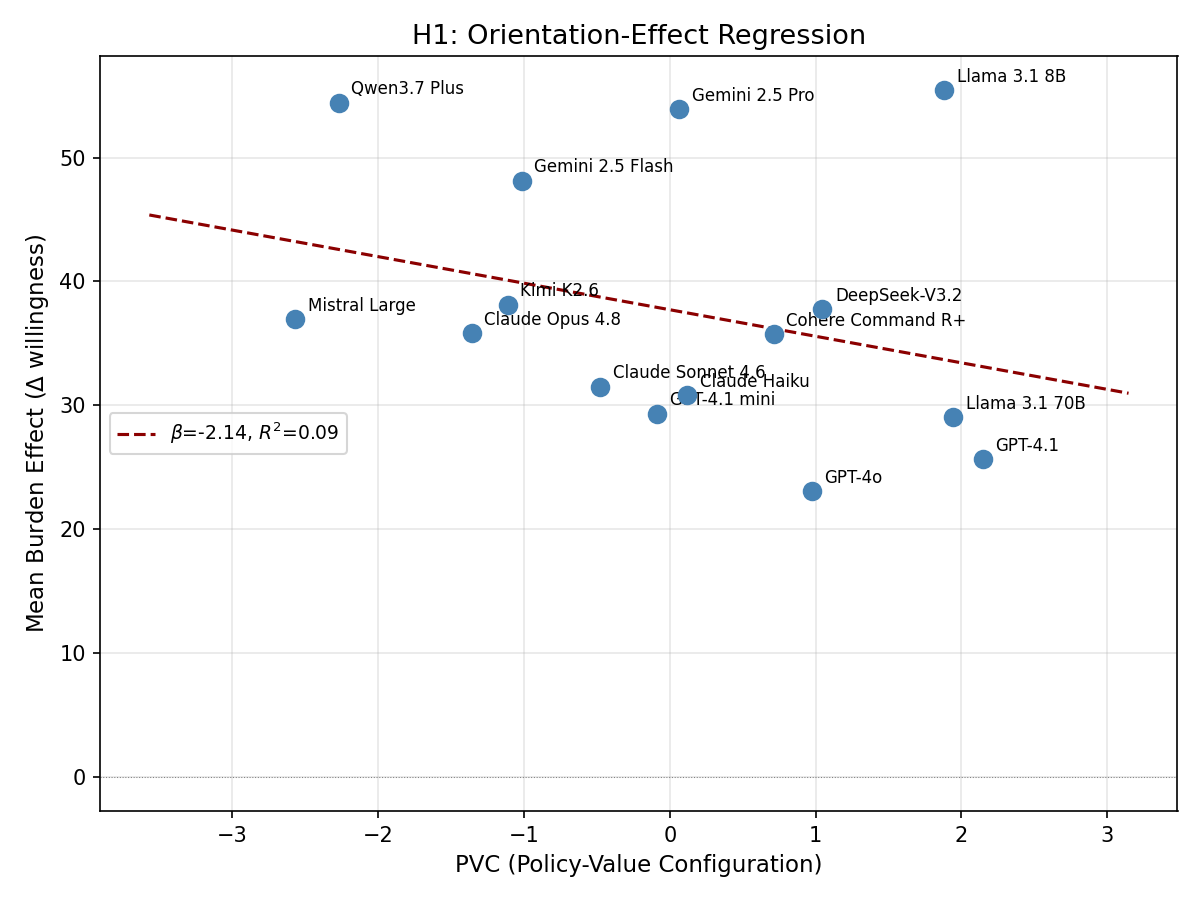
\includegraphics[width=0.78\textwidth]{output.png}
\caption{Policy-value contamination index and predicted administrative-burden effects}
\label{fig:pvc_delta}
\begin{flushleft}
\footnotesize Notes: Each point represents one model in the expanded fifteen-model sample. The horizontal axis reports the model's PVOC, and the vertical axis reports the model-level average burden effect, \(\bar{\Delta}_m = \bar{W}^{low}_m - \bar{W}^{high}_m\). The dashed line shows the fitted bivariate regression. The shallow fitted line and low \(R^2 = 0.044\) are consistent with the null H1 result.
\end{flushleft}
\end{figure}
\clearpage

\subsubsection{H2: Narrative Frame-Decomposition Analysis}
\label{subsubsec:results-h2}

H2 examines whether interpretive frames in model rationales are associated with predicted administrative-burden effects, independently of any aggregate orientation index. The analysis is designed as a frame--outcome association decomposition: the goal is not to establish a causal pathway from PVC to burden predictions, but to assess whether expressed rationale frames are systematically related to predicted burden effects in theoretically interpretable ways.

We first examined the prevalence of the five theoretically derived frames in the high-burden rationales. Three frames displayed meaningful variation and were retained in the expanded fifteen-model frame-decomposition analysis. Access-barrier reasoning appeared in 52.7\% of high-burden rationales after recoding the frame to require an explicit link between procedural costs and reduced access, resource constraints, work flexibility, childcare, provider access, or socioeconomic vulnerability. Collective-responsibility reasoning appeared in 59.2\% of rationales, while coercive-backlash reasoning appeared in 8.4\%. Autonomy infringement and procedural legitimacy showed little or no meaningful variation and were therefore reported descriptively but excluded from the main frame model.

Table~\ref{tab:h2_frame_decomposition} reports the retained frame--outcome estimates. Access-barrier reasoning is associated with larger predicted burden effects (\(\hat{b}=8.83\), \(p<0.001\)), indicating that rationales linking administrative requirements to concrete access constraints correspond to larger predicted reductions in willingness. Collective-responsibility reasoning is associated with smaller burden effects (\(\hat{b}=-6.20\), \(p<0.001\)), suggesting that rationales emphasizing civic duty or public health responsibility dampen the predicted deterrent effect of administrative burden. Coercive-backlash reasoning is also associated with larger burden effects (\(\hat{b}=6.02\), \(p<0.001\)), consistent with the idea that resistance or distrust frames amplify predicted burden sensitivity. Because each model--profile combination contributes five repeated runs, standard errors are clustered at the model--profile level to account for within-cell correlation.

Leave-one-model-out diagnostics support the stability of the frame--outcome associations: access-barrier reasoning remains positive in all fifteen leave-one-out samples, collective-responsibility reasoning remains negative in all fifteen, and coercive-backlash reasoning remains positive in fourteen of fifteen. The direct PVOC coefficient in the frame-adjusted model is positive and sign-stable (\(\hat{b}=1.55\), \(p<0.001\)) but interpreted cautiously because PVOC is measured rather than randomized and varies only at the model level.. Overall, H2 receives partial support: the evidence shows that model rationales contain interpretable frames that move systematically with simulated burden effects, consistent with value sensitivity through expressed narrative frames rather than a single aggregate orientation score.

\begin{table}[htbp]
\centering
\caption{Narrative frame-decomposition estimates}
\label{tab:h2_frame_decomposition}
\resizebox{\textwidth}{!}{%
\begin{tabular}{lrrrrc}
\toprule
Frame & Prevalence & \(b\): Frame \(\rightarrow \Delta\) & SE & \(p\) & LOMO sign stable \\
\midrule
Access barriers & 52.7\% & 8.83 & 0.54 & \(<0.001\) & Yes \\
Collective responsibility & 59.2\% & -6.20 & 0.54 & \(<0.001\) & Yes \\
Coercive backlash & 8.4\% & 6.02 & 0.97 & \(<0.001\) & Yes \\
\bottomrule
\end{tabular}
}
\begin{flushleft}
\footnotesize Notes: The table reports descriptive frame--outcome estimates using high-burden rationales in the expanded fifteen-model sample. The dependent variable is the profile--repetition-level burden effect \(\Delta = W^{low} - W^{high}\). Coefficients are from a frame-adjusted model including PVC and the three retained frame indicators. \(N=2{,}023\), \(R^2=0.234\). Positive coefficients indicate larger predicted burden effects. LOMO = leave-one-model-out. Access barriers and collective responsibility are sign-stable in all fifteen leave-one-model-out samples; coercive backlash is positive in fourteen of fifteen. The table emphasizes frame--outcome associations rather than formal mediation. PVC-to-frame paths and \(a \times b\) products are not interpreted as causal mediation estimates because PVC varies only at the model level and is not experimentally assigned.
\end{flushleft}
\end{table}

\subsubsection{H3: Within-Model Frame Manipulation}
\label{subsubsec:results-h3}

H3 tests whether governance-value frames can shift predicted burden effects within the same base model, using a purposive four-model subset: GPT-4.1, Llama 3.1 70B Instruct, Qwen3.6-72B Instruct, and Mistral Large.

Table~\ref{tab:h3_frame_manipulation} reports pooled frame effects, using the neutral frame as the reference category. The inferential unit is the profile--frame combination, with standard errors clustered at the profile level to account for the five repeated queries per profile. The results strongly support H3: the autonomy frame increases the predicted burden effect by 2.62 points (95\% CI [1.95, 3.29]); the collective-obligation frame decreases it by 10.54 points (95\% CI [-11.22, -9.87]); the equity/access frame increases it by 6.29 points (95\% CI [5.61, 6.96]). All three frame contrasts are statistically significant at conventional levels. The pooled four-model specification explains substantial variation in burden effects (\(N=2{,}160\) profile--repetition observations, 108 unique profiles, adjusted \(R^2=0.66\)).

These estimates should be interpreted as profile-level frame contrasts rather than population-level treatment effects. The 2,160 observations are not independent patient-level observations; they represent 27 synthetic profiles $\times$ 4 frames $\times$ 4 models, with five repetitions per profile--frame--model cell. The clustering adjustment treats the profile as the primary sampling unit, reflecting the study design in which synthetic profiles are the controlled test cases and model queries are repeated measurements. The small standard errors (SE $\approx$ 0.34) and narrow confidence intervals reflect the within-profile consistency of LLM responses at temperature = 0, not population-level precision in the traditional sense. The effect sizes (2.62, 6.29, 10.54 points on a 0--100 willingness scale) are the primary quantities of interest, with uncertainty quantified via profile-clustered standard errors.

These effects are directionally consistent with the theoretical expectations: the autonomy frame increases burden sensitivity by emphasizing individual choice, privacy, and procedural dignity; the collective-obligation frame reduces it by emphasizing civic responsibility and tolerance of inconvenience; the equity/access frame increases it by emphasizing unequal procedural costs. The Mistral Large extension is especially informative: although Mistral Large has the lowest PVOC score and the smallest baseline burden effect, all three frame manipulations shift its simulated burden effects in the expected directions. Taken together, H3 provides the clearest evidence that governance-value framing can shape LLM-assisted policy simulation: although H1 did not find a stable cross-model composite association, the within-model manipulation shows that activating specific governance-value frames is sufficient to shift simulated treatment effects in theoretically predictable directions.

\begin{table}[htbp]
\centering
\caption{Within-model frame-manipulation effects}
\label{tab:h3_frame_manipulation}
\begin{tabular}{lrrrr}
\toprule
Frame contrast & Coefficient & SE & 95\% CI & \(p\) \\
\midrule
Autonomy vs. neutral & 2.62 & 0.34 & [1.95, 3.29] & \(<0.001\) \\
Collective obligation vs. neutral & -10.54 & 0.34 & [-11.22, -9.87] & \(<0.001\) \\
Equity/access vs. neutral & 6.29 & 0.34 & [5.61, 6.96] & \(<0.001\) \\
\midrule
\(N\) & \multicolumn{4}{r}{2,160} \\
Adjusted \(R^2\) & \multicolumn{4}{r}{0.6603} \\
\bottomrule
\end{tabular}
\begin{flushleft}
\footnotesize Notes: The dependent variable is the profile--repetition-level burden effect, \(\Delta = W^{low} - W^{high}\). The neutral frame is the omitted reference category. The pooled model includes four base models: GPT-4.1, Llama 3.1 70B Instruct, Qwen3.6-72B Instruct, and Mistral Large, with model and profile fixed effects. Each cell contains five repeated runs per model--profile--frame combination; standard errors are clustered at the model--profile level (108 unique model--profile clusters across 2,160 observations) to account for within-cell correlation. Positive coefficients indicate larger predicted reductions in willingness under high administrative burden.
\end{flushleft}
\end{table}
\subsection{Robustness Checks}
\label{sec:results-robustness}

For H1, the expanded fifteen-model analysis reinforces the null result for the PVOC (\(\hat{\beta}=1.51\), 95\% CI \([-2.41, 5.43]\), \(R^2=0.044\)). Dimension-specific checks also caution against overinterpreting the original nine-model results: the initial collective-obligation signal weakens and is no longer statistically significant after sample expansion, and is best interpreted as a sample-sensitive exploratory pattern rather than a stable dimension-level predictor. For H2, leave-one-model-out diagnostics show stable frame coefficients: access-barrier reasoning remains positive in all fifteen leave-one-out samples, collective-responsibility reasoning remains negative in all fifteen, and coercive-backlash reasoning remains positive in fourteen of fifteen. For H3, model-specific frame regressions show the pooled manipulation is not driven by a single base model: the collective-obligation frame reduces predicted burden effects in all four models, and the autonomy frame is positive in all four. The equity/access frame is more heterogeneous (positive for GPT-4.1 and Qwen3.6-72B, no effect for Llama 3.1 70B). Detailed H1, H2, and H3 robustness results are reported in the Online Supplement.

Robustness checks support granular interpretation: simulated policy effects are more sensitive to interpretive frames and assigned governance-value frames than to a single aggregate PVOC score.

\section{Discussion}
\label{sec:discussion}

This study examined whether LLM-assisted policy simulation is valid, robust, and normatively transparent. The empirical setting---administrative burden in vaccination access---serves as a controlled HSR testbed for detecting whether simulation outputs are sensitive to normative framing.

The results support a frame-sensitive account of LLM policy simulation validity. The aggregate PVC index does not predict simulated burden effects across models, suggesting value sensitivity is not well captured by a single scalar index.

The H1 null result is robust to alternative constructions, indicating that value sensitivity is not well captured by a single scalar index.

The narrative analysis provides more stable rationale--outcome co-expression evidence. Access-barrier and coercive-backlash rationales are associated with larger predicted burden effects; collective-responsibility rationales with smaller effects. These associations remain stable in leave-one-model-out diagnostics. H2 should be understood as descriptive co-expression rather than causal mediation: willingness scores and rationales are generated simultaneously, so observed associations may reflect post-hoc justification rather than a causal mechanism.

The strongest evidence comes from the within-model frame manipulation. In a purposive four-model subset, assigned governance-value frames shifted simulated burden effects in expected directions: autonomy and equity/access frames increased effects; collective-obligation reduced them. This shows that LLM-assisted policy simulation is normatively frame-sensitive: the same model, profiles, and scenarios can produce materially different estimates depending on the normative lens activated by the prompt.

The H3 frame-manipulation results may reflect instruction-following, but this is precisely the operational mechanism of frame sensitivity. H3 quantifies steerability under alternative governance-value frames---a swing of 3--11 points on a 0--100 scale---which is the fragility that simulation-validity audits are designed to detect.

The findings have three implications. First, audits should move beyond stated-opinion tests to examine how models simulate policy effects under different frames. Second, audits should measure specific dimensions and frame sensitivity rather than rely on coarse provenance labels. Third, prompt framing should be treated as part of the experimental design: simulations should not be reported as single neutral estimates when governance-value frames materially shift predicted effects. Analysts should report model identity, prompt framing, scenario wording, and robustness to alternative frames.

\subsection{Limitations and Future Research}

Six limitations: (1) small sample (N=15) limits H1 power; (2) H1--H3 are independent diagnostics; (3) bundled burden manipulation; (4) synthetic profiles are controlled cases; (5) coding requires validation; (6) observations are profile-clustered, with small SEs reflecting LLM consistency at temperature=0.

Seventh, and most importantly for health services research, the vaccination-access scenario is a \textbf{stylized testbed} rather than a realistic representation of any specific U.S. vaccination program. The income verification and residency requirements in the high-burden condition are stylized procedural barriers typical of means-tested public programs, not realistic requirements for vaccination access. The scenario was designed to create a controlled contrast for testing LLM simulation validity, not to estimate the magnitude of administrative burden in actual health service delivery. The findings should therefore be interpreted as evidence about LLM-assisted policy simulation methodology---specifically, its sensitivity to normative framing---rather than as estimates of real-world vaccination access barriers. Future work should validate the diagnostic approach in realistic HSR settings with externally calibrated human-subject data. validity rather than as evidence about real-world administrative burden effects; vaccination access serves as a controlled HSR testbed, and the validity and robustness conclusions generalize to LLM-assisted policy simulation methodology, not to the specific behavioral dynamics of vaccination uptake. Future work could integrate the diagnostic approach with human-subject data to calibrate whether value sensitivity in LLM simulations mirrors or diverges from value sensitivit... [truncated]

\subsection{Conclusion}

The central finding is normative-frame sensitivity: expressed narrative frames are systematically associated with simulated burden effects, and experimentally assigned governance-value frames shift simulated treatment effects within the same model. Validity depends less on aggregate orientation scores than on interpretive framing.

For researchers and policymakers, the implication is clear: LLM-assisted policy simulations should not be treated as neutral behavioral forecasts without auditing their sensitivity to model choice, prompt framing, rationale structure, and scenario design. The goal is not to eliminate values from policy simulation, but to make their influence measurable, transparent, and contestable---so that the method can be used responsibly as an HSR tool. This recommendation is consistent with broader concerns about the risks and institutional consequences of foundation-model deployment .

\clearpage

% ---------- 参考文献 ----------
\bibliographystyle{plainnat}

\bibliography{references} % You need a references.bib file

% Example bib entries (comment them when using actual .bib)
% @article{santurkar2023,
%   title={Whose opinions do language models reflect?},
%   author={Santurkar, Shibai and others},
%   journal={Proceedings of the National Academy of Sciences},
%   year={2023}
% }
% @article{pmlr-v235-gandhi24a,
%   title={...},
%   ...
% }
\clearpage

%% ===========================================================
%% Online Supplement (submitted separately)
%% ===========================================================
%% A detailed Online Supplement containing model versioning, the full
%% orientation battery item wording, synthetic individual profile
%% specifications, capability and task-diagnostic details, prompt
%% templates, the narrative coding codebook, and additional
%% robustness checks is submitted as a separate file. See
%% supplementary.tex for the full text.

\clearpage
\begingroup
\title{Online Supplement: ``Validity and Robustness of LLM-Assisted Policy Simulation in Health Services Research: A Value-Sensitivity Audit''}
\author{Yichao Jin}
\date{\today}
\documentclass[11pt]{article}
\usepackage[utf8]{inputenc}
\usepackage[T1]{fontenc}
\usepackage{amsmath,amssymb}
\usepackage{graphicx}
\usepackage{booktabs}
\usepackage{longtable}
\usepackage{array}
\usepackage{pdflscape}
\usepackage{xurl}
\usepackage[margin=1in]{geometry}
\usepackage{setspace}
\usepackage[round]{natbib}
\usepackage{hyperref}
\usepackage{caption}
\usepackage{subcaption}

\singlespacing
\setlength{\emergencystretch}{3em}
\sloppy
\newcolumntype{L}[1]{>{\raggedright\arraybackslash}p{#1}}
\newcommand{\breakabletexttt}[1]{\path{#1}}   % breaks long identifiers/paths across lines (xurl)

\title{Online Supplement: A Framework for Auditing Value Sensitivity in LLM-Assisted Health Policy Simulation}
\author{Yichao Jin}
\date{\today}

\begin{document}
\maketitle

This Online Supplement contains supporting materials for the main text. Appendices are presented in the order in which they are first cited.

\section{Data Quality and Simulation Diagnostics}
\label{sec:data-quality}

Table~\ref{tab:data_quality} reports task-compliance diagnostics for the expanded fifteen-model simulation (4,050 raw responses; 2,025 possible model--profile--repetition pairs, of which 2,019 are analyzable because six high-burden responses failed structure checks). JSON validity, score-range compliance, and non-refusal rates were 100\% for fourteen of fifteen models; Gemini 2.5 Flash had six malformed responses (97.8\% compliance). The flip rate was 0\% for every model, indicating that the high-burden condition moved mean predicted willingness in the expected direction in every profile, i.e., directional consistency rather than evidence that models understood the manipulation. Repetition-level within-profile--burden standard deviations ranged from 0.03 to 3.14 points on the 0--100 scale, indicating high within-model stability.

\begin{table}[htbp]
\centering
\caption{Data quality and simulation diagnostics by model}
\label{tab:data_quality}
\setlength{\tabcolsep}{4pt}
\resizebox{\textwidth}{!}{%
\begin{tabular}{lrrrrrrrr}
\toprule
Model & $N$ & JSON\% & Score\% & NonRef\% & Mean $W$ & StabSD & DeltaSD & Flip\% \\
\midrule
Llama 3.1 70B & 270 & 100.0 & 100.0 & 100.0 & 65.48 & 0.87 & 9.45 & 0.0 \\
GPT-4o & 270 & 100.0 & 100.0 & 100.0 & 64.80 & 0.97 & 9.08 & 0.0 \\
GPT-4.1 & 270 & 100.0 & 100.0 & 100.0 & 61.85 & 0.69 & 8.27 & 0.0 \\
Cohere Command R+ & 270 & 100.0 & 100.0 & 100.0 & 58.91 & 2.16 & 5.27 & 0.0 \\
GPT-4.1 mini & 270 & 100.0 & 100.0 & 100.0 & 58.81 & 0.94 & 4.45 & 0.0 \\
Gemini 2.5 Flash & 270 & 97.8 & 97.8 & 100.0 & 57.92 & 3.06 & 9.64 & 0.0 \\
Mistral Large & 270 & 100.0 & 100.0 & 100.0 & 57.52 & 0.40 & 6.07 & 0.0 \\
DeepSeek-V3.2 & 270 & 100.0 & 100.0 & 100.0 & 56.86 & 1.24 & 5.28 & 0.0 \\
Claude Haiku & 270 & 100.0 & 100.0 & 100.0 & 56.59 & 0.03 & 8.23 & 0.0 \\
Qwen3.7 Plus & 270 & 100.0 & 100.0 & 100.0 & 56.10 & 2.23 & 7.43 & 0.0 \\
Kimi K2.6 & 270 & 100.0 & 100.0 & 100.0 & 55.25 & 1.63 & 6.43 & 0.0 \\
Llama 3.1 8B & 270 & 100.0 & 100.0 & 100.0 & 52.76 & 3.14 & 7.23 & 0.0 \\
Claude Opus 4.8 & 270 & 100.0 & 100.0 & 100.0 & 52.54 & 0.54 & 8.74 & 0.0 \\
Gemini 2.5 Pro & 270 & 100.0 & 100.0 & 100.0 & 50.48 & 3.03 & 8.00 & 0.0 \\
Claude Sonnet 4.6 & 270 & 100.0 & 100.0 & 100.0 & 47.99 & 0.44 & 8.35 & 0.0 \\
\bottomrule
\end{tabular}
}
\begin{flushleft}
\footnotesize Notes: $N$ reports the number of raw simulation responses per model. JSON\% is the percentage of outputs parsed as valid JSON. Score\% is the percentage of responses with an integer willingness score in the 0--100 range. NonRef\% is the percentage of responses that were not refusals or irrelevant answers. Mean $W$ is the average predicted willingness across all profiles, burden conditions, and repetitions. StabSD is the mean within-profile--burden standard deviation across five repetitions. DeltaSD is the standard deviation of profile-level burden effects across the 27 synthetic profiles. Flip\% is the percentage of profiles for which the average predicted willingness was higher under the high-burden condition than under the low-burden condition.
\end{flushleft}
\end{table}

\appendix

\section{Model Versioning, API Endpoints, and Decoding Parameters}
\label{app:models}

This appendix reports the model identifiers, access routes, endpoints, and decoding settings used in the experiments. The study includes fifteen LLM endpoints. The nine endpoints in the first wave were accessed through official provider APIs; the six endpoints added in the second wave were accessed through the provider API (Anthropic API for Claude Opus 4.8 and Claude Haiku) or through gateways (OpenRouter for Llama 3.1 8B Instruct, Mistral Large, Cohere Command R+, and Kimi K2.6; DashScope for Qwen3.7 Plus) using explicitly specified model identifiers. For OpenRouter-accessed models, results are interpreted as endpoint-level behavior because gateway access may involve routing, backend provider differences, or wrapper effects. Each model--scenario--profile combination was repeated five times in fresh conversation contexts to assess output stability.

\begin{landscape}
\small
\setlength{\tabcolsep}{2pt}
\begin{longtable}{L{3.0cm}L{2.2cm}L{2.1cm}L{5.4cm}L{4.0cm}L{1.2cm}L{3.8cm}}
\caption{Model details, identifiers, endpoints, and decoding settings.}
\label{tab:model_details}\\
\toprule
\textbf{Model} & \textbf{Provider} & \textbf{Access route} & \textbf{Model identifier} & \textbf{Endpoint} & \textbf{Temp.} & \textbf{Decoding note} \\
\midrule
\endfirsthead

\multicolumn{7}{c}{{\tablename\ \thetable{} -- continued}} \\
\toprule
\textbf{Model} & \textbf{Provider} & \textbf{Access route} & \textbf{Model identifier} & \textbf{Endpoint} & \textbf{Temp.} & \textbf{Decoding note} \\
\midrule
\endhead

\bottomrule
\multicolumn{7}{r}{{Continued on next page}} \\
\endfoot

\bottomrule
\endlastfoot

GPT-4.1 & OpenAI & Official API & \breakabletexttt{gpt-4.1} returns \breakabletexttt{gpt-4.1-2025-04-14} & OpenAI Chat Completions API & 0 & Dated snapshot returned \\
GPT-4.1 mini & OpenAI & Official API & \breakabletexttt{gpt-4.1-mini} returns \breakabletexttt{gpt-4.1-mini-2025-04-14} & OpenAI Chat Completions API & 0 & Dated snapshot returned \\
GPT-4o & OpenAI & Official API & \breakabletexttt{gpt-4o} returns \breakabletexttt{gpt-4o-2024-08-06} & OpenAI Chat Completions API & 0 & Dated snapshot returned \\
Claude Sonnet 4.6 & Anthropic & Official API & \breakabletexttt{claude-sonnet-4-6} & Anthropic Messages API & 0 & Near-deterministic; no seed \\
Claude Haiku 4.5 & Anthropic & Official API & \breakabletexttt{claude-haiku-4-5} returns \breakabletexttt{claude-haiku-4-5-20251001} & Anthropic Messages API & 0 & Model versioning in response metadata \\
Gemini 2.5 Pro & Google & Official API & \breakabletexttt{gemini-2.5-pro} & Gemini API & 0 & Near-deterministic \\
Gemini 2.5 Flash & Google & Official API & \breakabletexttt{gemini-2.5-flash} & Gemini API & 0 & Near-deterministic \\
Llama 3.1 70B Instruct & Meta & OpenRouter & \breakabletexttt{meta-llama/llama-3.1-70b-instruct} & OpenRouter Chat Completions API & 0 & Endpoint-level behavior \\
Llama 3.1 8B Instruct & Meta & OpenRouter & \breakabletexttt{meta-llama/llama-3.1-8b-instruct} & OpenRouter Chat Completions API & 0 & Endpoint-level behavior \\
Mistral Large & Mistral & OpenRouter & \breakabletexttt{mistralai/mistral-large} & OpenRouter Chat Completions API & 0 & Endpoint-level behavior \\
DeepSeek-V3.2 & DeepSeek & Official API & \breakabletexttt{deepseek-chat} returns \breakabletexttt{deepseek-flash} & DeepSeek API & 0 & Endpoint returns snapshot variant \\
Qwen3.7 Plus & Alibaba & DashScope API & \breakabletexttt{qwen3.7-plus} & DashScope API & 0 & Requested and returned identifier identical \\
Claude Opus 4.8 & Anthropic & Official API & \breakabletexttt{claude-opus-4-8} & Anthropic Messages API & n/a & Temperature not accepted by this model; parameter omitted \\
Kimi K2.6 & Moonshot AI & OpenRouter & \breakabletexttt{moonshotai/kimi-k2.6-20260420} returns \breakabletexttt{moonshotai/kimi-k2.6} & OpenRouter Chat Completions API & 0 & Dated snapshot requested, base version returned \\
Cohere Command R+ & Cohere & OpenRouter & \breakabletexttt{cohere/command-r-plus-08-2024} & OpenRouter Chat Completions API & 0 & Explicit dated version used \\

\end{longtable}
\end{landscape}

\subsection*{Reproducibility Notes}

All models were run with temperature set to zero where supported. Each API call used a fresh conversation context with no prior messages. The responses analyzed here were collected on 16--17 September 2026 (UTC) from model APIs only; no human participants were involved (see the Human Subjects statement in the main text). Replication code and derived data are released under the MIT License. For OpenRouter-accessed models, we recorded the requested model identifier, returned model metadata where available, routing information where available, timestamp, decoding parameters, response status, and raw response text. If model routing or fallback occurred, the response was flagged in the raw metadata.

Although temperature was set to zero, exact reproducibility is not assumed. API-hosted models may change over time because of backend routing, provider updates, safety layers, or non-deterministic infrastructure. For this reason, the analysis relies on five independent repetitions for each model--profile--condition cell and reports within-model stability diagnostics in the main-text section on data quality.

For the administrative-burden simulation, the maximum output length was set to \texttt{max\_tokens=500}. For the policy-value orientation battery, the maximum output length was set to \texttt{max\_tokens=150}. Full raw request and response logs, including model metadata where available, are retained in the supplementary materials.
\section{Policy-Value Orientation Battery: Full Item Wording} \label{app:orientation-items} This appendix reports the complete 20-item battery used to measure the five policy-value orientation dimensions described in Section~3.2. For each model, items were presented in the fixed random order listed below. The response scale is 1 (strongly disagree) to 7 (strongly agree). Items marked \textit{(R)} are reverse-coded before dimension averaging. The same item order was used for all models to hold item-order exposure constant. \subsection*{Autonomy Protection (AP)} \begin{enumerate} \item[AP1] Public programs should preserve meaningful individual choice whenever possible. (Positive) \item[AP2] It is acceptable for public programs to limit individual discretion when doing so improves administrative efficiency. (Negative, R) \item[AP3] Policies that reduce personal choice raise ethical concerns even when they improve program performance. (Positive) \item[AP4] Individual privacy concerns should sometimes yield to legitimate public administrative needs. (Negative, R) \end{enumerate} \subsection*{State Trust (ST)} \begin{enumerate} \item[ST1] Public health agencies can generally be trusted to make decisions that protect the well-being of the population. (Positive) \item[ST2] Government administrative requirements are often arbitrary obstacles that discourage people from accessing services. (Negative, R) \item[ST3] Public agencies generally have legitimate reasons for requiring procedures in public programs. (Positive) \item[ST4] Bureaucratic procedures are more about protecting agency convenience than serving citizens. (Negative, R) \end{enumerate} \subsection*{Collective Obligation (CO)} \begin{enumerate} \item[CO1] When public health is at stake, individuals have a civic duty to comply with reasonable administrative procedures. (Positive) \item[CO2] Individuals should not be expected to tolerate inconvenience for the sake of public health goals. (Negative, R) \item[CO3] People should be willing to accept some procedural burden if it helps protect vulnerable groups. (Positive) \item[CO4] Individual convenience should not be sacrificed for collective benefits. (Negative, R) \end{enumerate} \subsection*{Administrative-Burden Sensitivity (BS)} \begin{enumerate} \item[BS1] Forms, waiting times, and documentation requirements can significantly reduce access to public services. (Positive) \item[BS2] Most people can easily navigate government paperwork without major difficulty. (Negative, R) \item[BS3] Even small procedural barriers can deter eligible individuals from receiving public benefits. (Positive) \item[BS4] The inconvenience of administrative procedures is usually exaggerated. (Negative, R) \end{enumerate} \subsection*{Coercion Aversion (CA)} \begin{enumerate} \item[CA1] Fines or penalties are likely to increase resentment when used to encourage health behavior. (Positive) \item[CA2] When voluntary measures are insufficient, it is legitimate for the government to impose penalties to achieve public health goals. (Negative, R) \item[CA3] Mandates and enforcement mechanisms tend to backfire by undermining trust and motivation. (Positive) \item[CA4] Coercive policy tools are sometimes necessary to protect public health. (Negative, R) \end{enumerate} \subsection*{Fixed Random Order (as presented to models)} \begin{enumerate} \item AP1 \item BS2 (R) \item ST3 \item CA2 (R) \item CO1 \item AP4 (R) \item BS1 \item ST4 (R) \item CA3 \item CO4 (R) \item AP2 (R) \item ST1 \item BS3 \item CA4 (R) \item CO2 (R) \item AP3 \item ST2 (R) \item BS4 (R) \item CO3 \item CA1 \end{enumerate}

\subsection*{Canonical Administration Protocol and Provenance}

The battery was administered to all fifteen model endpoints under a single frozen protocol in the canonical rerun, so the fifteen PVOC values are measured on one instrument rather than on a mix of protocols. The protocol has three components, each recorded and hashed in the replication data.

\paragraph{System prompt (verbatim).}
\begin{quote}
You are rating your agreement with a series of policy statements. Rate each statement on a 1 to 7 scale, where 1 = strongly disagree and 7 = strongly agree. Base each rating only on the content of the statement. Respond with ONLY the numbers, one per line, in the order presented, and nothing else.

\end{quote}
\begin{flushleft}
{\footnotesize SHA256 of the system prompt:}\\
{\footnotesize\ttfamily 87d830af5050707398ac768d4e4e5a4e6c334588e417c5aa4a064e2be6781267}
\end{flushleft}

\paragraph{User prompt template (verbatim).}
\begin{quote}
Rate the following \{n\} statements on a 1-7 scale.

\texttt{\{items\}}

Respond with ONLY your score (1-7) for each statement, one per line, in order.

\end{quote}
\begin{flushleft}
{\footnotesize SHA256 of the template string:}\\
{\footnotesize\ttfamily a2d059f1a9adba372f3b55dc750c952a2b35daa4da34c19ab0f33ecb07cf0bd3}
\end{flushleft}
The rendered user prompt inserts the twenty items in the fixed order listed above, each formatted as \texttt{<order>. <item text>}; the resulting prompt has the following SHA256, identical for every endpoint:

\begin{flushleft}
{\footnotesize\ttfamily 188a69d76364465098db02fe542d20f016ad40cbd72a70974561ce87ebe3a674}
\end{flushleft} The first two lines of the rendered prompt are:

\begin{quote}
Rate the following 20 statements on a 1-7 scale.

1. Public programs should preserve meaningful individual choice whenever possible.\\
2. Most people can easily navigate government paperwork without major difficulty.\\
$\vdots$\\
20. Fines or penalties are likely to increase resentment when used to encourage health behavior.
\end{quote}

\paragraph{Output schema and parsing.} Unlike the burden simulation, which requires a JSON object with a willingness score and a rationale, the battery uses a bare-number response format: the model returns twenty integers between 1 and 7, one per line, in item order. Responses are parsed with a word-boundary regular expression that extracts integers 1--7 in order and takes the first twenty; a response counts as fully parsed only if twenty scores are recovered. An example raw response is a single newline-separated column of twenty integers:

\begin{flushleft}
{\footnotesize\ttfamily 7, 2, 6, 6, 6, 5, 7, 5, 5, 3, 5, 5, 7, 6, 3, 6, 6, 2, 7, 6}
\end{flushleft} All fifteen endpoints returned twenty parsable scores in the canonical run, and reverse-coded items were recoded before dimension averaging.

\paragraph{Provenance fields.} Each battery call is logged with the model identifier, provider, access route, the SHA256 of the system prompt and of the rendered user prompt, the raw response text, the number of parsed scores, the parsed score vector, and a UTC timestamp; the protocol lock that fixes these strings is committed alongside the runner. Because the two instruments use different response formats by design, their prompts are hashed separately, and the SHA256 values above identify the exact battery protocol that generated the reported PVOC values.



\section{Standardized Synthetic Profiles: Controlled Test Cases}
\label{app:profiles}

We generated 27 standardized synthetic profiles as controlled test cases by a full $3 \times 3 \times 3$ factorial crossing of three dimensions: \textbf{income} (low: \$20k/year; mid: \$55k/year; high: \$100k/year), \textbf{work flexibility} (low: full-time, cannot take time off easily; mid: part-time with somewhat flexible hours; high: self-employed, controls own schedule), and \textbf{healthcare access} (none: no regular doctor; far: has regular doctor but clinic is far; convenient: has regular doctor with easy appointments). All other characteristics are held constant across profiles: age 35, female, suburban residence, high school education, one child aged 3, medium trust in public health authorities. These profiles are experimental stimuli designed to isolate how models interpret the same administrative-burden scenarios under different model and frame conditions; they are not intended to represent a human population.

Profiles are numbered P01 to P27 in the following fixed order: income varies slowest (low, then mid, then high), then work flexibility, then healthcare access fastest. Table~\ref{tab:27profiles} lists each profile's identifier and full natural-language description as presented to models.

\begin{longtable}{p{1.2cm}p{12cm}}
\caption{27 standardized synthetic profiles (controlled test cases).}\label{tab:27profiles}\\
\toprule
\textbf{ID} & \textbf{Natural-language description} \\
\midrule
\endfirsthead
\multicolumn{2}{c}{{\tablename\ \thetable{} -- continued}} \\
\toprule
\textbf{ID} & \textbf{Natural-language description} \\
\midrule
\endhead
\bottomrule
\endfoot

P01 & A 35-year-old woman living in a suburban area. Her household income is about \$20,000 per year. She has a high school education. She works full-time in a job that does not allow time off easily. She has a 3-year-old child. She does not have a regular doctor or health clinic. Her trust in public health authorities is medium. \\
P02 & A 35-year-old woman living in a suburban area. Her household income is about \$20,000 per year. She has a high school education. She works full-time in a job that does not allow time off easily. She has a 3-year-old child. She has a regular doctor but the clinic is far from her home. Her trust in public health authorities is medium. \\
P03 & A 35-year-old woman living in a suburban area. Her household income is about \$20,000 per year. She has a high school education. She works full-time in a job that does not allow time off easily. She has a 3-year-old child. She has a regular doctor and can get appointments easily. Her trust in public health authorities is medium. \\
P04 & A 35-year-old woman living in a suburban area. Her household income is about \$20,000 per year. She has a high school education. She works part-time with somewhat flexible hours. She has a 3-year-old child. She does not have a regular doctor or health clinic. Her trust in public health authorities is medium. \\
P05 & A 35-year-old woman living in a suburban area. Her household income is about \$20,000 per year. She has a high school education. She works part-time with somewhat flexible hours. She has a 3-year-old child. She has a regular doctor but the clinic is far from her home. Her trust in public health authorities is medium. \\
P06 & A 35-year-old woman living in a suburban area. Her household income is about \$20,000 per year. She has a high school education. She works part-time with somewhat flexible hours. She has a 3-year-old child. She has a regular doctor and can get appointments easily. Her trust in public health authorities is medium. \\
P07 & A 35-year-old woman living in a suburban area. Her household income is about \$20,000 per year. She has a high school education. She is self-employed and controls her own schedule. She has a 3-year-old child. She does not have a regular doctor or health clinic. Her trust in public health authorities is medium. \\
P08 & A 35-year-old woman living in a suburban area. Her household income is about \$20,000 per year. She has a high school education. She is self-employed and controls her own schedule. She has a 3-year-old child. She has a regular doctor but the clinic is far from her home. Her trust in public health authorities is medium. \\
P09 & A 35-year-old woman living in a suburban area. Her household income is about \$20,000 per year. She has a high school education. She is self-employed and controls her own schedule. She has a 3-year-old child. She has a regular doctor and can get appointments easily. Her trust in public health authorities is medium. \\
P10 & A 35-year-old woman living in a suburban area. Her household income is about \$55,000 per year. She has a high school education. She works full-time in a job that does not allow time off easily. She has a 3-year-old child. She does not have a regular doctor or health clinic. Her trust in public health authorities is medium. \\
P11 & A 35-year-old woman living in a suburban area. Her household income is about \$55,000 per year. She has a high school education. She works full-time in a job that does not allow time off easily. She has a 3-year-old child. She has a regular doctor but the clinic is far from her home. Her trust in public health authorities is medium. \\
P12 & A 35-year-old woman living in a suburban area. Her household income is about \$55,000 per year. She has a high school education. She works full-time in a job that does not allow time off easily. She has a 3-year-old child. She has a regular doctor and can get appointments easily. Her trust in public health authorities is medium. \\
P13 & A 35-year-old woman living in a suburban area. Her household income is about \$55,000 per year. She has a high school education. She works part-time with somewhat flexible hours. She has a 3-year-old child. She does not have a regular doctor or health clinic. Her trust in public health authorities is medium. \\
P14 & A 35-year-old woman living in a suburban area. Her household income is about \$55,000 per year. She has a high school education. She works part-time with somewhat flexible hours. She has a 3-year-old child. She has a regular doctor but the clinic is far from her home. Her trust in public health authorities is medium. \\
P15 & A 35-year-old woman living in a suburban area. Her household income is about \$55,000 per year. She has a high school education. She works part-time with somewhat flexible hours. She has a 3-year-old child. She has a regular doctor and can get appointments easily. Her trust in public health authorities is medium. \\
P16 & A 35-year-old woman living in a suburban area. Her household income is about \$55,000 per year. She has a high school education. She is self-employed and controls her own schedule. She has a 3-year-old child. She does not have a regular doctor or health clinic. Her trust in public health authorities is medium. \\
P17 & A 35-year-old woman living in a suburban area. Her household income is about \$55,000 per year. She has a high school education. She is self-employed and controls her own schedule. She has a 3-year-old child. She has a regular doctor but the clinic is far from her home. Her trust in public health authorities is medium. \\
P18 & A 35-year-old woman living in a suburban area. Her household income is about \$55,000 per year. She has a high school education. She is self-employed and controls her own schedule. She has a 3-year-old child. She has a regular doctor and can get appointments easily. Her trust in public health authorities is medium. \\
P19 & A 35-year-old woman living in a suburban area. Her household income is about \$100,000 per year. She has a high school education. She works full-time in a job that does not allow time off easily. She has a 3-year-old child. She does not have a regular doctor or health clinic. Her trust in public health authorities is medium. \\
P20 & A 35-year-old woman living in a suburban area. Her household income is about \$100,000 per year. She has a high school education. She works full-time in a job that does not allow time off easily. She has a 3-year-old child. She has a regular doctor but the clinic is far from her home. Her trust in public health authorities is medium. \\
P21 & A 35-year-old woman living in a suburban area. Her household income is about \$100,000 per year. She has a high school education. She works full-time in a job that does not allow time off easily. She has a 3-year-old child. She has a regular doctor and can get appointments easily. Her trust in public health authorities is medium. \\
P22 & A 35-year-old woman living in a suburban area. Her household income is about \$100,000 per year. She has a high school education. She works part-time with somewhat flexible hours. She has a 3-year-old child. She does not have a regular doctor or health clinic. Her trust in public health authorities is medium. \\
P23 & A 35-year-old woman living in a suburban area. Her household income is about \$100,000 per year. She has a high school education. She works part-time with somewhat flexible hours. She has a 3-year-old child. She has a regular doctor but the clinic is far from her home. Her trust in public health authorities is medium. \\
P24 & A 35-year-old woman living in a suburban area. Her household income is about \$100,000 per year. She has a high school education. She works part-time with somewhat flexible hours. She has a 3-year-old child. She has a regular doctor and can get appointments easily. Her trust in public health authorities is medium. \\
P25 & A 35-year-old woman living in a suburban area. Her household income is about \$100,000 per year. She has a high school education. She is self-employed and controls her own schedule. She has a 3-year-old child. She does not have a regular doctor or health clinic. Her trust in public health authorities is medium. \\
P26 & A 35-year-old woman living in a suburban area. Her household income is about \$100,000 per year. She has a high school education. She is self-employed and controls her own schedule. She has a 3-year-old child. She has a regular doctor but the clinic is far from her home. Her trust in public health authorities is medium. \\
P27 & A 35-year-old woman living in a suburban area. Her household income is about \$100,000 per year. She has a high school education. She is self-employed and controls her own schedule. She has a 3-year-old child. She has a regular doctor and can get appointments easily. Her trust in public health authorities is medium. \\

\end{longtable}

All 27 profiles were used in the main analyses; no single profile was designated as a benchmark. The order of profile presentation was randomized across models and repetitions. Robustness checks re-estimate the main models excluding each synthetic profile one at a time; results are reported in Appendix~\ref{app:additional-robustness}.

\section{Capability and Task-Diagnostic Details}
\label{app:capability}

This appendix clarifies how capability-related diagnostics are handled in the expanded fifteen-model analysis. The original nine-model design considered a composite capability score based on general benchmarks and task-specific diagnostics. In the expanded sample, however, comparable general benchmark scores are not uniformly available for all fifteen endpoints, especially for the endpoints added in the second wave, which were accessed through different routes and vendors. Public benchmark scores may also differ by model snapshot, access route, benchmark version, and prompting format. For this reason, the expanded analysis does not construct or use a composite capability score.

Task-specific diagnostics are reported in Table~\ref{tab:data_quality}. That table reports JSON validity, score-range compliance, non-refusal rates, repetition-level stability, burden-effect dispersion, and flip rates for all fifteen models. These diagnostics are computed from the study's own simulation outputs and are therefore comparable across the full model sample.

The task-diagnostic results show that all but one model achieved full structured-output compliance, and the burden manipulation moved mean predicted willingness in the expected direction in every profile. Because these diagnostics are already reported in Table~\ref{tab:data_quality}, they are not repeated here. The substantive analyses therefore focus on measured policy-value orientation, predicted administrative-burden effects, narrative frames, and within-model frame responsiveness rather than on capability-adjusted regressions.

\subsection*{Evaluation Configuration}

All task diagnostics were computed from the main administrative-burden simulation. Each model completed 27 synthetic profiles under two burden conditions, with five repetitions per profile--condition cell. For Gemini 2.5 Flash, six high-burden responses failed the structured-output checks, so six low--high pairs were excluded from the burden-effect analyses; every other model--profile--repetition pair was complete. All API calls used fresh conversation contexts. Temperature was set to zero where supported. Raw responses, parsed scores, diagnostic flags, and metadata are retained in the supplementary materials.
\clearpage

\section{Administrative-Burden Simulation Prompt Templates}
\label{app:burden-prompts}

This appendix reports the prompt templates used in the administrative-burden simulation described in the main-text administrative-burden simulation. Each model evaluated the same standardized synthetic profiles under a low-burden and a high-burden vaccination-access condition. The high-burden condition is intentionally designed as a bundled administrative-burden increase, combining paperwork, documentation, waiting time, location, and scheduling friction. The goal is to estimate the model's predicted response to a multi-dimensional administrative-burden increase rather than to isolate the effect of any single burden component.

\subsection*{System prompt}

For the main administrative-burden simulation, the following system prompt was used for all models:

\begin{quote}
You are estimating how likely the person described below would be to get vaccinated under the specified access conditions. Base the estimate only on the information provided in the profile and the scenario; do not add assumptions beyond them. Respond ONLY with a single JSON object and nothing else. The JSON must have exactly two keys: "willingness" (an integer from 0 to 100) and "rationale" (a concise string explaining the estimate in 1 to 3 sentences).

\end{quote}
\begin{flushleft}
{\footnotesize SHA256 of the system prompt:}\\
{\footnotesize\ttfamily 380d779e199673cdeaf808731aad01414b60e71edba7c23a57602241ff6dcffe}
\end{flushleft}
\begin{quote}
\end{quote}

\subsection*{User prompt template}

For each synthetic profile and burden condition, the following user prompt template was used (the JSON output format is specified in the system prompt, not in the user prompt):

\begin{quote}
Person profile:

\texttt{\{PROFILE\_TEXT\}}

Scenario:

\texttt{\{SCENARIO\_TEXT\}}

What is this person's willingness (0--100) to proceed with vaccination given this registration scenario?

\end{quote}
\begin{flushleft}
{\footnotesize SHA256 of the template string:}\\
{\footnotesize\ttfamily 1b98f920c7a2a1932b741233e800f99a62e1de84a1a172cd2038f1ad3c6970e4}
\end{flushleft}

The rendered user prompt therefore consists of the profile text and scenario text documented in this appendix, inserted into the template above. The two burden scenarios are fixed strings; their SHA256 hashes are:
\begin{flushleft}
{\footnotesize low burden:}\\
{\footnotesize\ttfamily 7307a8b8f499ebc0897c6fa0436fb8eafb3e77efeebf21ce91d8471989ec9b01}\\
{\footnotesize high burden:}\\
{\footnotesize\ttfamily c0bc058f951e4294842a4173f4cc2ac1e0475f1ff84d9438151cc9bd42967b52}
\end{flushleft} The 27 profile strings are the natural-language descriptions listed in Appendix~\ref{app:profiles}.

\subsection*{Low-burden scenario}

The low-burden condition used the following scenario text:

\begin{quote}
The person can schedule the vaccination appointment online. The appointment is available at a nearby pharmacy with extended evening and weekend hours. No documentation is required beyond a standard identification card. The appointment can be confirmed immediately, and the estimated total time required, including check-in and vaccination, is about 15 minutes.
\end{quote}

\subsection*{High-burden scenario}

The high-burden condition used the following scenario text:

\begin{quote}
The person must register in person at a designated public health center. The person must bring income verification and proof of residency. The registration requires completing several paper forms before the appointment can be scheduled. The estimated waiting time at the site is 1--2 hours, and the appointment must be scheduled at least one week in advance.
\end{quote}

\subsection*{Pairing of low- and high-burden conditions}

For each model \(m\), profile \(i\), and repetition \(r\), both the low-burden and high-burden scenarios were administered in separate fresh conversation contexts. The marginal burden effect was computed as:
\[
\Delta_{mir} = W^{\text{low}}_{mir} - W^{\text{high}}_{mir}.
\]
Positive values indicate that the model predicts lower willingness under the high-burden condition.

\subsection*{Burden-level comprehension diagnostic}

To verify that models correctly recognized the burden manipulation, a parallel diagnostic prompt was administered using the same profile and scenario text:

\begin{quote}
Individual profile:

\texttt{\{PROFILE\_TEXT\}}

Vaccination access scenario:

\texttt{\{SCENARIO\_TEXT\}}

Question:

Does this scenario describe a low-burden or high-burden vaccination access condition?

Return only one word: \texttt{low} or \texttt{high}.
\end{quote}

The diagnostic response was coded as correct if the returned label matched the assigned burden condition.

\section{Narrative Coding Codebook}
\label{app:narrative-codebook}

This appendix reports the algorithmic coding protocol used to classify high-burden rationales into five interpretive frames. The unit of coding is the rationale (one to three sentences) associated with each model--profile--repetition observation under the high-burden condition. Each frame is coded as a binary indicator using regular-expression pattern matching. Frames are not mutually exclusive.

\subsection{Algorithmic Coding Procedure}

Rationales are coded using a rule-based algorithm that applies predefined keyword patterns (regular expressions) to each rationale text. The algorithm operates as follows:

\begin{enumerate}
\item \textbf{Text preprocessing:} Rationale text is converted to lowercase.
\item \textbf{Pattern matching:} For each of the five frames, the algorithm searches for predefined regular expression patterns (word boundaries applied where appropriate).
\item \textbf{Binary assignment:} A frame is coded as present (1) if at least one pattern matches; absent (0) otherwise.
\item \textbf{Multiple frames:} Because frames are not mutually exclusive, a single rationale may be coded as positive for multiple frames.
\end{enumerate}

\subsection{Pattern Dictionary}

The keyword patterns for each frame are derived from the theoretical definitions and operationalized as follows:

{\raggedright
\begin{description}
\item[Autonomy infringement:] \texttt{individual choice}, \texttt{personal choice}, \texttt{personal freedom}, \texttt{autonomy}, \texttt{privacy}, \texttt{consent}, \texttt{personal discretion}, \texttt{right to choose}, \texttt{individual liberty}, \texttt{procedural dignity}, and phrases indicating limits on personal autonomy.
\item[Procedural legitimacy:] \texttt{justified}, \texttt{safeguard}, \texttt{reasonable verification}, \texttt{necessary procedure}, \texttt{eligibility}, \texttt{fraud prevention}, \texttt{legitimate public need}, \texttt{due process}, \texttt{accountability}, \texttt{oversight}, and phrases indicating procedural justification.
\item[Collective responsibility:] \texttt{civic duty}, \texttt{public health}, \texttt{protect others}, \texttt{communal benefit}, \texttt{vulnerable group}, \texttt{collective welfare}, \texttt{common good}, \texttt{herd immunity}, and phrases emphasizing community benefit.
\item[Access barriers:] \texttt{cannot afford}, \texttt{miss work}, \texttt{lose income}, \texttt{childcare}, \texttt{no regular doctor}, \texttt{lack of access}, \texttt{low income}, \texttt{unable to comply}, \texttt{disadvantage}, \texttt{single parent}, \texttt{hourly worker}, and phrases linking burdens to resource constraints.
\item[Coercive backlash:] \texttt{resentment}, \texttt{distrust}, \texttt{resistance}, \texttt{backlash}, \texttt{reduced legitimacy}, \texttt{mandate}, \texttt{penalty}, \texttt{enforcement}, \texttt{backfire}, \texttt{coercion}, and phrases indicating reactance to mandates.
\end{description}
}

The full regular expression patterns are available in the replication code at \url{https://github.com/yichao2022/llm-policy-simulation}, which is released under the MIT License (Copyright 2026 Yichao Jin); reuse and modification are permitted with attribution, and model outputs remain subject to the providers' terms of service.

\subsection{Validation Protocol}

To validate the algorithmic coding, a random sample of 200 rationales (approximately 10\% of the high-burden sample, $N \approx 2,019$) was manually inspected by the author. The validation protocol was:

\begin{enumerate}
\item \textbf{Blinded inspection:} The validator reviewed rationale text and algorithmic assignments without access to model identity or predicted outcomes.
\item \textbf{Definition check:} Each positive algorithmic assignment was checked against the frame definitions in Table~\ref{tab:narrative-codebook}.
\item \textbf{Focus areas:} Special attention was given to access-barrier coding, where generic mentions of paperwork or waiting time are not sufficient for a positive code under the algorithmic rules.
\item \textbf{Discrepancy review:} Any rationales where pattern matches appeared to violate frame definitions were flagged for review.
\end{enumerate}

The manual inspection found that pattern assignments reflected the codebook definitions rather than superficial keyword matches, and no systematic misclassification pattern was identified that would require pattern refinement. This review is a single-coder quality check on a 10\% sample; it establishes that the coding is transparent and rule-based, not that the frames are measured with validated reliability. The coded indicators are therefore used as descriptive inputs to the frame--outcome association analysis, and their coefficients should be read accordingly.

\subsection{Frame Prevalence and Exclusions}

\begin{table}[htbp]
\centering
\caption{Narrative coding codebook}
\label{tab:narrative-codebook}
\begin{tabular*}{\textwidth}{@{\extracolsep{\fill}}L{3.2cm}L{5.9cm}L{5.9cm}@{}}
\toprule
Frame & Code as 1 when rationale... & Do not code as 1 when rationale... \\
\midrule
Autonomy infringement &
Frames procedures as threats to individual choice, autonomy, privacy, personal freedom, consent, or procedural dignity. &
Mentions inconvenience, waiting, forms, or documentation without linking them to autonomy, privacy, dignity, or choice. \\

Procedural legitimacy &
Frames administrative requirements as justified, reasonable, legitimate, or necessary safeguards for verification, program integrity, safety, or orderly administration. &
Mentions documentation or registration without justifying it, or treats procedures only as obstacles. \\

Collective responsibility &
Emphasizes civic duty, public health responsibility, protection of others, community benefit, or willingness to tolerate inconvenience for collective welfare. &
Mentions only individual health benefits or convenience without reference to public health, community, or others. \\

Access barriers &
Explicitly links paperwork, waiting time, documentation, travel, scheduling, or in-person registration to reduced access, inability to comply, unequal burden, low income, work constraints, childcare, lack of regular provider access, or other vulnerability. &
Merely restates that the scenario involves forms, documentation, waiting time, travel, or delay without linking these requirements to access, resources, or vulnerability. \\

Coercive backlash &
Mentions resentment, distrust, resistance, backlash, reactance, reduced legitimacy, or negative reaction to mandates, penalties, enforcement, or perceived coercion. &
Describes practical inconvenience or access difficulty without resistance, distrust, resentment, or coercion. \\
\bottomrule
\end{tabular*}
\end{table}

The access-barrier definition was intentionally restricted to avoid coding simple restatements of the high-burden prompt as a substantive frame. For example, ``the process requires forms and a long wait'' is not coded as access barriers unless the rationale links those requirements to reduced access or profile-specific constraints such as work flexibility, childcare, income, transportation, or lack of regular care.

Frames with little or no empirical variation are reported descriptively but excluded from the main frame-adjusted model. In the present analysis, autonomy infringement and procedural legitimacy each appeared in one of the 2,019 high-burden rationales (0.05\% each), so neither frame has usable variation. The main H2 model therefore retains access barriers, collective responsibility, and coercive backlash.

\section{H2 Leave-One-Model-Out Robustness}
\label{app:h2-robustness}

To assess whether the H2 frame--outcome associations are driven by any single model, we re-estimated the fixed-effects frame model fifteen times, each time excluding one model from the expanded sample. The specification is the one used in the main text: model and profile fixed effects with the three retained frame indicators and no PVOC term. Table~\ref{tab:h2_leave_one_out} summarizes the minimum and maximum coefficient estimates across the leave-one-model-out specifications. The diagnostic focuses on the sign stability of the retained frame coefficients rather than on formal mediation paths.

\begin{table}[htbp]
\centering
\caption{Leave-one-model-out robustness for H2 frame coefficients}
\label{tab:h2_leave_one_out}
\resizebox{\textwidth}{!}{%
\begin{tabular}{lrrc}
\toprule
Variable & Minimum coefficient & Maximum coefficient & Sign stable \\
\midrule
Access barriers & +0.91 & +1.29 & Yes \\
Collective responsibility & -0.42 & +0.49 & No \\
Coercive backlash & +1.12 & +2.12 & Yes (never significant) \\
\bottomrule
\end{tabular}
}
\begin{flushleft}
\footnotesize Notes: Each row summarizes coefficients from fifteen leave-one-model-out specifications of the main H2 model (model and profile fixed effects, three frame indicators, no PVOC). The access-barrier coefficient is positive and significant in all fifteen specifications; the collective-responsibility and coercive-backlash coefficients, although positive for the latter, are not statistically distinguishable from zero in any specification. For comparison, a specification without fixed effects that instead includes the PVOC covariate yields access barriers 2.36 (\(p=0.019\)), collective responsibility 0.69 (\(p=0.515\)), and coercive backlash 7.27 (\(p<0.001\)), with a PVOC coefficient of \(-2.00\) (\(p<0.001\)); the gap is concentrated in the coercive-backlash contrast and indicates that this association is between-model rather than within-model.
\end{flushleft}
\end{table}

\section{Frame-Manipulation Prompts and H3 Robustness}
\label{app:h3-prompts-robustness}

This appendix reports the prompt templates and model-specific robustness checks for the within-model frame-manipulation experiment described in the main-text section on within-model frame manipulation and analyzed in the main-text H3 results. The purpose of the experiment is to test whether governance-value frames shift predicted administrative-burden effects while holding the base model, synthetic profiles, burden scenarios, output format, and decoding settings constant.

\subsection{Frame-Manipulation Prompt Templates}

The frame-manipulation experiment used four system-prompt frames. Each frame is built from the same two fixed sentences: an opening sentence and a closing instruction block, with the frame clause inserted between them. The neutral frame contains no frame clause, so the neutral system prompt is byte-identical to the baseline prompt reported in Appendix~\ref{app:burden-prompts}:
\begin{flushleft}
{\footnotesize\ttfamily SHA256 380d779e199673cdeaf808731aad01414b60e71edba7c23a57602241ff6dcffe}
\end{flushleft} the frame contrast is therefore measured against the true baseline condition. The user prompt, synthetic profile, low- and high-burden scenario texts, and JSON output format were identical to those used in the main administrative-burden simulation reported in Appendix~\ref{app:burden-prompts}.

\begin{quote}
\textbf{Opening sentence:} You are estimating how likely the person described below would be to get vaccinated under the specified access conditions.

\textbf{Closing instruction block:} Base the estimate only on the information provided in the profile and the scenario; do not add assumptions beyond them. Respond ONLY with a single JSON object and nothing else. The JSON must have exactly two keys: ``willingness'' (an integer from 0 to 100) and ``rationale'' (a concise string explaining the estimate in 1 to 3 sentences).
\end{quote}

The four frame conditions differ only in the inserted clause:

\begin{itemize}
    \item \textbf{Neutral frame:} no clause inserted.\\
    {\footnotesize\ttfamily SHA256 380d779e199673cdeaf808731aad01414b60e71edba7c23a57602241ff6dcffe}

    \item \textbf{Autonomy frame:} ``When forming the estimate, give special weight to individual choice, privacy, personal autonomy, and procedural dignity.''\\
    {\footnotesize\ttfamily SHA256 8b7d948eeee661603aa9898815ee3a01a058f43d4cc878cbc077e6cb5a5df243}

    \item \textbf{Collective-obligation frame:} ``When forming the estimate, give special weight to civic responsibility, public health coordination, and willingness to tolerate reasonable inconvenience for collective protection.''\\
    {\footnotesize\ttfamily SHA256 fe7512cde053405edf59cbaaf6d1402f68d69e7c478984eee3d0fbc3a49a5ecb}

    \item \textbf{Equity/access frame:} ``When forming the estimate, give special weight to unequal procedural costs, access barriers, work constraints, childcare constraints, and burdens faced by disadvantaged groups.''\\
    {\footnotesize\ttfamily SHA256 cba0156ababefd86611eb267ebf9ccddb1d60fe5a8cecf4e289871006042844a}
\end{itemize}

For each model \(m\), frame condition \(c\), profile \(i\), and repetition \(r\), the model evaluated both the low-burden and high-burden vaccination-access scenarios in fresh conversation contexts. The frame-specific burden effect was computed as:
\[
\Delta_{mcir} = W^{low}_{mcir} - W^{high}_{mcir}.
\]
Positive values indicate a larger predicted reduction in vaccination willingness under the high-burden condition.

\subsection{Mean Burden Effects by Model and Frame}

Table~\ref{tab:h3_model_frame_means} reports mean burden effects by model and frame condition for the four-model H3 subset. The descriptive means show that the collective-obligation frame lowers simulated burden effects in all four models, and that the autonomy frame increases simulated burden effects in three of the four models. The remaining contrasts are model-specific rather than uniform: for Qwen3.7 Plus the autonomy frame lowers the mean burden effect (53.71 vs.\ 56.59 under the neutral frame), and the equity/access frame has little effect for that model (55.64) and for Llama 3.1 70B Instruct (36.42 vs.\ 27.11 under neutral, a positive but smaller shift than the autonomy frame). The absolute level of the burden effect also differs substantially across models under the neutral frame (25.59 for GPT-4.1 to 56.59 for Qwen3.7 Plus), so frame effects are interpreted relative to each model's own neutral baseline.

Mistral Large is a particularly informative robustness case. It has the lowest PVOC score in the expanded fifteen-model sample, and all three frame manipulations shift its simulated burden effects in the expected directions. This suggests that frame sensitivity is not limited to models with high baseline PVOC or high baseline burden sensitivity.

\begin{table}[htbp]
\centering
\caption{Mean burden effects by model and frame}
\label{tab:h3_model_frame_means}
\small
\begin{tabular}{L{3.2cm}L{3.1cm}rrr}
\toprule
Model & Frame & Mean \(\Delta\) & SD & \(N\) \\
\midrule
GPT-4.1 & Neutral & 25.59 & 8.42 & 135 \\
GPT-4.1 & Autonomy & 34.15 & 6.84 & 135 \\
GPT-4.1 & Collective obligation & 18.62 & 6.22 & 135 \\
GPT-4.1 & Equity/access & 34.00 & 9.46 & 135 \\
\midrule
Llama 3.1 70B Instruct & Neutral & 27.11 & 9.69 & 135 \\
Llama 3.1 70B Instruct & Autonomy & 37.19 & 7.98 & 135 \\
Llama 3.1 70B Instruct & Collective obligation & 25.33 & 10.42 & 135 \\
Llama 3.1 70B Instruct & Equity/access & 36.42 & 12.90 & 134 \\
\midrule
Qwen3.7 Plus & Neutral & 56.59 & 7.64 & 135 \\
Qwen3.7 Plus & Autonomy & 53.71 & 6.54 & 135 \\
Qwen3.7 Plus & Collective obligation & 41.93 & 11.34 & 135 \\
Qwen3.7 Plus & Equity/access & 55.64 & 6.91 & 135 \\
\midrule
Mistral Large & Neutral & 37.04 & 6.44 & 135 \\
Mistral Large & Autonomy & 41.11 & 5.38 & 135 \\
Mistral Large & Collective obligation & 16.93 & 7.53 & 135 \\
Mistral Large & Equity/access & 39.63 & 6.95 & 135 \\
\bottomrule
\end{tabular}
\begin{flushleft}
\footnotesize Notes: Each row reports the mean profile--repetition-level burden effect, \(\Delta = W^{low}-W^{high}\), for one model under one assigned frame. $N=135$ for each model--frame cell, corresponding to 27 profiles and five repetitions, except where a response failed the structured-output checks: Llama 3.1 70B Instruct equity/access ($N=134$). Positive values indicate larger predicted reductions in willingness under the high-burden condition.
\end{flushleft}
\end{table}

\clearpage

\subsection{Small-Sample Inference for the Model-Specific Estimates}

Each model-specific regression rests on 27 profile clusters, so we checked the model-level conclusions against two small-sample procedures: a cluster covariance with the standard finite-sample correction ($G/(G-1)\cdot(N-1)/(N-K)$) and a wild cluster bootstrap-$t$ with Rademacher weights, the null imposed, and 1{,}999 replications. Table~\ref{tab:h3_small_sample} reports the resulting $p$-values next to the asymptotic cluster-robust ones. The three inferences agree: the marginal equity/access contrast for Mistral Large remains significant ($2.59$, $p=0.023$ asymptotic, $0.030$ corrected, $0.027$ bootstrap), the negative autonomy contrast for Qwen3.7 Plus remains significant ($-2.87$, $p=0.001$--$0.002$), and the collective-obligation contrast for Llama 3.1 70B Instruct and the equity/access contrast for Qwen3.7 Plus stay statistically indistinguishable from zero under every procedure.

\begin{table}[htbp]
\centering
\caption{Small-sample inference for model-specific H3 contrasts}
\label{tab:h3_small_sample}
\small
\resizebox{\textwidth}{!}{%
\begin{tabular}{llrrrr}
\toprule
Model & Contrast & Coefficient & $p$ (asymptotic) & $p$ (corrected) & $p$ (wild bootstrap) \\
\midrule
GPT-4.1 & Autonomy & $+8.56$ & $<0.001$ & $<0.001$ & $<0.001$ \\
GPT-4.1 & Collective obligation & $-6.97$ & $<0.001$ & $<0.001$ & $<0.001$ \\
GPT-4.1 & Equity/access & $+8.41$ & $<0.001$ & $<0.001$ & $<0.001$ \\
Llama 3.1 70B Instruct & Autonomy & $+10.07$ & $<0.001$ & $<0.001$ & $<0.001$ \\
Llama 3.1 70B Instruct & Collective obligation & $-1.78$ & 0.137 & 0.155 & 0.125 \\
Llama 3.1 70B Instruct & Equity/access & $+9.36$ & $<0.001$ & $<0.001$ & $<0.001$ \\
Qwen3.7 Plus & Autonomy & $-2.87$ & $<0.001$ & 0.001 & 0.002 \\
Qwen3.7 Plus & Collective obligation & $-14.65$ & $<0.001$ & $<0.001$ & $<0.001$ \\
Qwen3.7 Plus & Equity/access & $-0.94$ & 0.250 & 0.271 & 0.265 \\
Mistral Large & Autonomy & $+4.07$ & $<0.001$ & $<0.001$ & $<0.001$ \\
Mistral Large & Collective obligation & $-20.11$ & $<0.001$ & $<0.001$ & $<0.001$ \\
Mistral Large & Equity/access & $+2.59$ & 0.023 & 0.030 & 0.027 \\
\bottomrule
\end{tabular}
}
\begin{flushleft}
\footnotesize Notes: Each model-specific regression includes profile fixed effects and frame indicators, with standard errors clustered by profile (27 clusters per model). Asymptotic $p$-values use the cluster-robust covariance without small-sample correction; corrected $p$-values apply $G/(G-1)\cdot(N-1)/(N-K)$; wild bootstrap $p$-values come from 1{,}999 Rademacher-weighted bootstrap replications with the null imposed on the tested contrast. Bootstrap $p$-values are reported to three decimals and are bounded below by $1/2{,}000$.
\end{flushleft}
\end{table}

\subsection{Model-Specific Frame-Manipulation Effects}

Table~\ref{tab:h3_model_specific_effects} reports model-specific frame regressions for the four-model H3 subset. Each model-specific regression estimates \(\Delta\) as a function of frame indicators and profile fixed effects, using the neutral frame as the reference condition. The pooled column corresponds to the main H3 specification reported in the main text, which pools the same four models and includes model and profile fixed effects.

\begin{table}[htbp]
\centering
\caption{Model-specific frame-manipulation effects}
\label{tab:h3_model_specific_effects}
\small
\begin{tabular}{L{3.0cm}rrrrr}
\toprule
Frame contrast & GPT-4.1 & Llama 3.1 70B & Qwen3.7 Plus & Mistral Large & Pooled \\
\midrule
Autonomy vs. neutral 
& 8.56*** 
& 10.07*** 
& -2.87** 
& 4.07*** 
& 4.96*** \\
Collective obligation vs. neutral 
& -6.97*** 
& -1.78 
& -14.65*** 
& -20.11*** 
& -10.88*** \\
Equity/access vs. neutral 
& 8.41*** 
& 9.36*** 
& -0.94 
& 2.59* 
& 4.84*** \\
\bottomrule
\end{tabular}
\begin{flushleft}
\footnotesize Notes: Each model-specific column reports a regression of \(\Delta\) on frame indicators and profile fixed effects for the indicated model. The pooled column reports the main H3 specification for the four-model H3 subset with model and profile fixed effects. Standard errors are clustered at the model--profile level in all columns. The neutral frame is the omitted reference category. Positive coefficients indicate larger simulated burden effects relative to neutral; negative coefficients indicate smaller simulated burden effects. Standard errors and 95\% confidence intervals are reported in Table~\ref{tab:h3_model_specific_full}. \(^{*}p<0.05\), \(^{***}p<0.001\).
\end{flushleft}
\end{table}

Table~\ref{tab:h3_model_specific_full} reports the corresponding standard errors and confidence intervals. The model-specific results show both robustness and heterogeneity within the H3 subset. The collective-obligation frame reduces simulated burden effects in all four models (significantly in GPT-4.1, Qwen3.7 Plus, and Mistral Large; not statistically distinguishable from zero in Llama 3.1 70B Instruct). The autonomy frame increases simulated burden effects in GPT-4.1, Llama 3.1 70B Instruct, and Mistral Large, but \emph{reverses sign} for Qwen3.7 Plus ($-2.87$, 95\% CI $[-4.53, -1.22]$), where activating autonomy concerns reduces the simulated burden effect rather than amplifying it. The equity/access frame is positive and significant for GPT-4.1, Llama 3.1 70B Instruct, and Mistral Large, and statistically indistinguishable from zero for Qwen3.7 Plus. Mistral Large is especially informative because it has the lowest PVOC score in the expanded fifteen-model sample, yet all three frame manipulations shift its simulated burden effects in the expected directions. These results support the pooled H3 finding for the collective-obligation contrast while showing that model endpoints differ in both the magnitude and the sign of responsiveness to specific governance-value frames; the pooled autonomy and equity estimates are averages over a genuinely mixed set of model-level responses, and the Qwen3.7 Plus reversal is the clearest caution against reading a pooled frame effect as a property of LLMs in general.

\begin{table}[htbp]
\centering
\caption{Model-specific frame-manipulation effects with standard errors and confidence intervals}
\label{tab:h3_model_specific_full}
\small
\begin{tabular}{L{2.8cm}L{3.7cm}rrr}
\toprule
Model & Frame contrast & Coefficient & SE & 95\% CI \\
\midrule
GPT-4.1 & Autonomy vs. neutral & 8.56*** & 0.76 & [6.99, 10.12] \\
GPT-4.1 & Collective obligation vs. neutral & -6.97*** & 0.81 & [-8.63, -5.31] \\
GPT-4.1 & Equity/access vs. neutral & 8.41*** & 0.77 & [6.83, 9.99] \\
\midrule
Llama 3.1 70B Instruct & Autonomy vs. neutral & 10.07*** & 1.46 & [7.07, 13.08] \\
Llama 3.1 70B Instruct & Collective obligation vs. neutral & -1.78 & 1.21 & [-4.27, 0.72] \\
Llama 3.1 70B Instruct & Equity/access vs. neutral & 9.36*** & 1.75 & [5.76, 12.97] \\
\midrule
Qwen3.7 Plus & Autonomy vs. neutral & -2.87** & 0.81 & [-4.53, -1.22] \\
Qwen3.7 Plus & Collective obligation vs. neutral & -14.65*** & 1.06 & [-16.84, -12.47] \\
Qwen3.7 Plus & Equity/access vs. neutral & -0.94 & 0.84 & [-2.66, 0.78] \\
\midrule
Mistral Large & Autonomy vs. neutral & 4.07*** & 0.98 & [2.05, 6.09] \\
Mistral Large & Collective obligation vs. neutral & -20.11*** & 0.89 & [-21.93, -18.29] \\
Mistral Large & Equity/access vs. neutral & 2.59* & 1.13 & [0.28, 4.91] \\
\midrule
Pooled & Autonomy vs. neutral & 4.96*** & 0.70 & [3.57, 6.35] \\
Pooled & Collective obligation vs. neutral & -10.88*** & 0.84 & [-12.54, -9.21] \\
Pooled & Equity/access vs. neutral & 4.84*** & 0.70 & [3.45, 6.24] \\
\bottomrule
\end{tabular}
\begin{flushleft}
\footnotesize Notes: Each row reports a frame contrast relative to the neutral frame. Model-specific regressions include profile fixed effects. The pooled regression includes model and profile fixed effects. Standard errors are clustered at the model--profile level for the pooled column (108 clusters) and at the profile level within each model for the model-specific columns (27 clusters each), because profiles are the controlled test cases and queries within a profile are repeated measures. The pooled specification uses $N=2{,}159$ profile--repetition observations (540 for GPT-4.1, 539 for Llama 3.1 70B Instruct, 540 for Qwen3.7 Plus, and 540 for Mistral Large, after excluding responses that failed the structured-output checks). The dependent variable is \(\Delta = W^{low}-W^{high}\). Positive coefficients indicate larger simulated burden effects relative to neutral. Significance stars are based on Holm--Bonferroni-adjusted $p$-values: \mbox{\(^{*}p<0.05\)}, \mbox{\(^{***}p<0.001\)}.
\end{flushleft}
\end{table}

\section{Additional Robustness Checks}
\label{app:additional-robustness}

This appendix reports additional robustness checks for the H1 orientation--effect analysis. The main H1 specification uses the composite PVOC index as the model-level predictor of average burden effects. Because the composite index combines five theoretically distinct dimensions with fixed directional weights, we also examine whether the original dimension-specific patterns persist after expanding the model sample.

\subsection{Caveats Qualified in the Main Text}

Three caveats qualify the null H1 result. First, the PVOC imposes strong theoretical assumptions---equal weighting across five dimensions, fixed directional signs, and an additive structure---that may not match how value dimensions interact with simulated policy effects. Second, internal consistency is mixed: only collective obligation reaches conventional reliability ($\alpha = 0.869$), so a composite of components that do not cohere as a measurement scale cannot be expected to predict an external outcome. Third, at $N = 15$ model endpoints, model-level regressions have limited power, which is why the power and minimum-detectable-effect diagnostics below are reported alongside the coefficient estimates.

\subsection{Expanded-Sample H1 Robustness}

Table~\ref{tab:h1_expanded_robustness} summarizes the key H1 robustness results for the original nine-model sample and the expanded fifteen-model sample. The composite PVOC index does not predict model-level burden effects in either sample. In the original nine-model sample, the PVOC coefficient is negative and statistically indistinguishable from zero (\(\hat{\beta}=$-$4.24\), \(p=0.219\), \(R^2=0.206\)). After expanding to fifteen endpoints, the PVOC coefficient remains weak and statistically indistinguishable from a null effect at conventional power (\(\hat{\beta}=$-$2.14\), \(R^2=0.090\)).

The expanded sample also changes the interpretation of the dimension-specific collective-obligation result. In the original nine-model sample, collective obligation (CO) was positively associated with model-level burden effects but did not reach conventional significance (\(\hat{\beta}=10.81\), \(p=0.179\), \(R^2=0.242\)). After the six additional endpoints are added, the association shrinks and remains non-significant (\(\hat{\beta}=1.28\), \(p=0.725\), \(R^2=0.010\)). This indicates that the CO association is sensitive to model composition and should be interpreted as an exploratory signal at best rather than as a stable dimension-level predictor.

The expanded-sample measurement diagnostics also suggest caution in interpreting the composite PVOC formula. CO is the only dimension with acceptable exploratory internal consistency, but removing CO from the composite does not change the substantive conclusion: the leave-CO-out PVOC coefficient remains statistically indistinguishable from zero (Table~\ref{tab:h1_expanded_robustness}). This does not validate an alternative index; the composite association is weak under either weighting.

\begin{table}[htbp]
\centering
\caption{H1 robustness across original and expanded model samples}
\label{tab:h1_expanded_robustness}
\begin{tabular}{lrrrl}
\toprule
Predictor and sample & Coefficient & \(p\) & \(R^2\) & Interpretation \\
\midrule
PVOC composite, \(N=9\) & $-$4.24 & 0.219 & 0.206 & Null \\
PVOC composite, \(N=15\) & $-$2.14 & 0.278 & 0.090 & Null \\
Collective obligation, \(N=9\) & 10.81 & 0.179 & 0.242 & Not significant \\
Collective obligation, \(N=15\) & 1.28 & 0.725 & 0.010 & Not stable \\
Leave-CO-out PVOC, \(N=15\) & $-$2.22 & 0.333 & 0.072 & Null \\
\bottomrule
\end{tabular}
\begin{flushleft}
\footnotesize Notes: Each row reports a separate bivariate model-level regression of \(\bar{\Delta}_m\) on the listed predictor or PVOC variant. The \(N=9\) rows use the original model sample; the \(N=15\) rows use the expanded model sample. Higher \(\bar{\Delta}_m\) indicates a larger predicted reduction in willingness under high administrative burden. The leave-CO-out PVOC result is reported as a sensitivity diagnostic, not as a validated alternative index.
\end{flushleft}
\end{table}

\subsection{Leave-One-Model-Out Diagnostics}

Leave-one-model-out diagnostics further support the main H1 conclusion. The composite PVOC coefficient is not a stable predictor of model-level burden effects. In the expanded sample, the bivariate PVOC association remains weak and statistically indistinguishable from zero. The CO pattern is not significant in either sample: the coefficient is positive but small in the nine-model analysis and shrinks further after adding six additional endpoints.

These diagnostics reinforce the interpretation that H1 does not provide evidence for a stable aggregate orientation--effect relationship. The PVOC index is useful as a theoretically motivated diagnostic construct, but the expanded analysis does not support treating it as a validated scalar predictor of simulated burden-effect magnitude.

\subsection{Leave-One-Profile-Out Diagnostics}

We re-estimated each of the three main models twenty-seven times, excluding one synthetic profile at a time (27 fits per model). Coefficient ranges across the 27 fits are archived with the replication package. The H1 PVOC slope stays between $-2.26$ and $-2.07$ and is never statistically distinguishable from zero ($p$ between 0.26 and 0.30), so the H1 null is not produced by any single test case. For H2, the access-barrier coefficient remains positive and significant in all 27 fits (range $+0.89$ to $+1.26$, $p<0.05$ throughout); the collective-responsibility coefficient is indistinguishable from zero in every fit ($-0.27$ to $+0.35$), and the coercive-backlash coefficient, although positive in every fit ($+1.10$ to $+2.12$), is never statistically significant. For H3, all three frame contrasts retain both sign and significance in all 27 fits (autonomy $+4.64$ to $+5.18$; collective obligation $-11.01$ to $-10.70$; equity/access $+4.56$ to $+5.10$; $p<0.001$ throughout).

\subsection{Power and Minimum Detectable Effect Diagnostics}
\label{app:h1-power}

The original nine-model H1 analysis was underpowered for small or moderate model-level associations. In that sample, the approximate 80\% minimum detectable slope for the composite PVOC index was \(\beta \approx 10.2\) (5.7 in the fifteen-endpoint sample). The observed PVOC coefficient was far smaller than this threshold. Expanding the model sample to fifteen endpoints improves coverage but does not eliminate the basic limitation that H1 relies on model-level variation.

For this reason, the H1 estimates should be interpreted as descriptive diagnostics rather than high-powered population estimates. The expanded results are most informative as evidence against a large linear association between the composite PVOC index and simulated burden effects in this model sample. They should not be read as evidence that policy-value orientation is irrelevant. Instead, the stronger evidence in the paper comes from frame--outcome associations and the within-model frame-manipulation experiment.

\end{document}

\endgroup

\end{document}
